\chapter{Esquemas de discretización numérica}
\label{cap:esquemas}

% http://math.sfsu.edu/beck/quotes.html
\begin{chapterquote}[0.87\linewidth]
\smallskip
\textit{CITA DE PIAGET - RUBBER DUCK DEBUGGING}
\end{chapterquote}

\noindent
Las formulaciones de los modelos matemáticos del transporte y difusión de neutrones en estado estacionario desarrollados en el capítulo anterior arrojan expresiones integro-diferenciales sobre seis escalares independientes: tres para el espacio~$\vec{x}$, dos para la dirección~$\omegaversor$ y uno para la energía~$E$. En este capítulo vamos a ir transformando estas dependencias y operadores continuos a versiones discretas para poder ser resueltas con computadoras digitales. Comenzamos primero por la energía aplicando la idea de grupos discretos de energías y continuamos por la dependencia angular con el método de ordenadas discretas~S$_N$, que sólo aplica a la formulación de transporte. Finalmente prestamos atención a la discretización espacial, que es el aporte principal de esta tesis al problema del análisis de reactores nucleares de potencia moderados por auga pesada. En este trabajo desarrollamos dos esquemas: uno basado en volúmenes finitos y otro basado en elementos finitos. Dejamos fuera de toda discusión a los esquemas basados en diferencias finitas porque si bien son los más sencillos de todoss, estos esquemas no pueden manejar discontinudades en las propiedades materiales ni mallas no estructuradas, que es el tema central de esta tesis.

Este capítulo podríamos haberlo organizado de dos maneras diferentes. La primera es desarrollar completamente~S$_N$, primero discertizando en energía, luego en ángulo y finalmente en el espacio, primero con volúmenes finitos y luego en elementos, para después pasar a estudiar completamente difusión comenzando con la energía y continuado con el espacio primero en volúmenes y finalmente en elementos finitos. La segunda es estudiar primero la discretización en energía para tanto para transporte como para difusión, luego analizar la discretización angular de transporte y pasar finalmente a la discretización espacial tanto de ordenadas discretas como de difusión primero con volúmenes finitos y luego terminar con transporte y difusión formuladas con elementos finitos. Elegimos la segunda organización.

\section{Discretización en energía}

Vamos a discretizar el dominio de la energía~$E$ utilizando el concepto clásico de física de reactores de \emph{grupos de energías}, que llevado a conceptos más generales de matemática discreta es equivalente a aplicar el método de volúmenes finitos, sólo que esta vez los volúmenes son volúmenes de energía. En efecto, tomemos el intervalo de energías~$[0,E_0]$ donde~$E_0$ es la mayor energía esperada de un neutrón individual. Como ilustramos en la figura~\ref{fig:multigroup}, dividamos dicho intervalo en~$G$ grupos (volúmenes) no necesariamente iguales cada uno definido por energías de corte~$0=E_G < E_{G-1} < \dots < E_2 < E_1 < E_0$, de forma tal que el grupo~$g$ es el intervalo~$[E_g,E_{g-1}]$. Notamos que con esta notación, el grupo número uno siempre es el de mayor energía. A medida que un neutrón va perdiendo energía, va aumentando el número de su grupo de energía.

\begin{figure}[h]
\begin{center}
\includegraphics[width=0.9\linewidth]{esquemas/multigroup-energy}
\end{center}
\caption{\label{fig:multigroup}Discretización del dominio energético en grupos (volúmenes) de energía. Tomamos la mayor energía esperada~$E_0$ y divididmos el intervalo~$[0,E_0]$ en~$G$ grupos, no necesariamente iguales. El esquema matemático es equivalente a una discretización por volúmenes finitos. El grupo uno es el de mayor energía.}
\end{figure}


El objetivo de discretizar la energía en~$G$ grupos es transformar la dependencia continua del flujo~$\psi(\vec{x}, \omegaversor, E)$ por~$G$ funciones~$\psi_g(\vec{x}, \omegaversor)$. De la misma manera, pasar de~$\phi(\vec{x}, E)$ a~$G$ funciones~$\phi_g(\vec{x})$.

\begin{definicion}\label{def:flujogrupo}
El flujo angular del grupo~$g$ es

\begin{equation}
 \psi_g(\vec{x}, \omegaversor) = \int_{E_g}^{E_{g-1}} \psi(\vec{x}, \omegaversor, E) \, dE
\end{equation}
%
y el flujo escalar del grupo~$g$ es

\begin{equation}
 \phi_g(\vec{x}) = \int_{E_g}^{E_{g-1}} \phi(\vec{x}, E) \, dE
\end{equation}

Notamos que~$\psi(\vec{x}, \omegaversor, E$ y~$\psi_g(\vec{x}, \omegaversor)$ no tienen las mismas unidades. La primera magnitud tiene unidades de inversa de área por inversa de ángulo sólido por inversa de energía por inversa de tiempo (i.e. $\text{cm}^{-2} \cdot \text{eV}^{-1} \cdot \text{s}^{-1}$, mientras que la segunda es un flujo integrado por lo que sus unidades son inversa de área por inversa de ángulo sólido por inversa de tiempo (i.e. $\text{cm}^{-2} \cdot \text{s}^{-1}$). La misma idea aplica a~$\phi(\vec{x}, E)$ y a~$\phi_g(\vec{x})$.
\end{definicion}

La idea de la discretización es re-escribir las ecuaciones de transporte y/o difusión en función de los flujos de grupo. Para fijar ideas, prestemos atención al término de absorción total de la ecuación de transporte~$\Sigma_t \cdot \psi$, e integrémoslo entre~$E_g$ y~$E_{g-1}$. Quisiéramos que esta integral sea igual al producto entre el flujo~$\psi_g$ y el valor medio de la sección eficaz total en dicho grupo:

\begin{equation*}
\int_{E_g}^{E_{g-1}} \Sigma_t(\vec{x}, E) \cdot \psi(\vec{x}, \omegaversor, E) \, dE =
\Sigma_{t g}(\vec{x}) \cdot \psi_g(\vec{x}, \omegaversor)
\end{equation*}

Está claro que para que esto sea posible, la sección eficaz total~$\Sigma_{t g}$ media en el grupo~$g$ debe ser

\begin{equation}\label{eq:sigmatg}
\Sigma_{t g}(\vec{x}) = \frac{\displaystyle \int_{E_g}^{E_{g-1}} \Sigma_t(\vec{x}, E) \cdot \psi(\vec{x}, \omegaversor, E) \, dE}{\displaystyle \int_{E_g}^{E_{g-1}} \psi(\vec{x}, \omegaversor, E) \, dE}
\end{equation}
%
con lo que no hemos ganado nada ya que llegamos a una condición tautológica donde el parámetro que necesitamos para no necesitar la dependencia explícita del flujo con la energía depende justamente de dicha dependencia. Sin embargo, y es ésta una de las ideas centrales del cálculo y análisis de reactores, podemos suponer que el cálculo de celda es capaz de proveernos las secciones eficaz macroscópicas multigrupo para el reactor que estamos modelando de forma tal que, desde el punto de vista del cálculo de núcleo, $\Sigma_{t g}$ y todas las demás secciones eficaces son distribuciones conocidas del espacio~$\vec{x}$.

% \medskip
Procediendo en forma análoga con la sección eficaz de fisión, tenemos que

\begin{equation}\label{eq:nusigmafg}
\nu\Sigma_{f g}(\vec{x}) = \frac{\displaystyle \int_{E_g}^{E_{g-1}} \nu\Sigma_f(\vec{x}, E) \cdot \psi(\vec{x}, \omegaversor, E) \, dE}{\displaystyle \int_{E_g}^{E_{g-1}} \psi(\vec{x}, \omegaversor, E) \, dE}
\end{equation}

Para el caso del término de scattering, la sección eficaz de scattering desde el ángulo~$\omegaprimaversor$ hacia el ángulo~$\omegaversor$ y desde el grupo de energía~$g^\prime$ hacia el grupo~$g$ es

\begin{equation}\label{eq:sigmasggprima}
\Sigma_{s g^\prime \rightarrow g}(\vec{x}, \omegaprimaversor \rightarrow \omegaversor) =
\frac{\displaystyle \int_{E_g}^{E_{g-1}} \int_{E^\prime_{g^\prime}}^{E^\prime_{g^\prime -1}}
\Sigma_{s}(\vec{x}, \omegaprimaversor \rightarrow \omegaversor, E^\prime \rightarrow E) \cdot \psi(\vec{x}, \omegaprimaversor, E^\prime) \, dE^\prime \, dE }
{\displaystyle \int_{E_g}^{E_{g-1}} \int_{E^\prime_{g^\prime}}^{E^\prime_{g^\prime -1}} \psi(\vec{x}, \omegaprimaversor, E^\prime) \, dE^\prime \, dE}
\end{equation}


\bigskip

Tomemos entonces el caso de medio multiplicativo con fuente de la sección~\ref{sec:multiplicativoconfuente} e integremos la ecuación de transporte~\eqref{eq:transportemmfi} sobre la energía~$E$ en el grupo~$g$, es decir en el intervalo~$E_g < E < E_{g-1}$:

\begin{multline*}
 \int_{E_g}^{E_{g-1}} \omegaversor \cdot \text{grad} \left[ \psi(\vec{x}, \omegaversor, E) \right] \, dE
 + \int_{E_g}^{E_{g-1}}  \Sigma_t(\vec{x}, E) \cdot \psi(\vec{x}, \omegaversor, E) \, dE = \\
 \int_{E_g}^{E_{g-1}}  \int_{0}^{\infty} \int_{4\pi} \Sigma_s(\vec{x}, \boldsymbol{\hat{\Omega}^\prime} \rightarrow \omegaversor, E^\prime \rightarrow E) \cdot \psi(\vec{x}, \boldsymbol{\hat{\Omega}^\prime}, E^\prime) \, d\boldsymbol{\hat{\Omega}^\prime} \, dE^\prime \, dE \\
+ \int_{E_g}^{E_{g-1}}  \frac{\chi(E)}{4\pi} \int_{0}^{\infty} \int_{4\pi} \nu\Sigma_f(\vec{x}, E^\prime) \cdot \psi(\vec{x}, \boldsymbol{\hat{\Omega}^\prime}, E^\prime) \, d\boldsymbol{\hat{\Omega}^\prime} \, dE^\prime \, dE
+ \int_{E_g}^{E_{g-1}}  s(\vec{x}, \omegaversor, E) \, dE
\end{multline*}

Utilizando la definición~\ref{def:flujogrupo} y reemplazando las ecuaciones~\eqref{eq:sigmatg}, \eqref{eq:nusigmafg} y~\eqref{eq:sigmasggprima}, obtenemos a las~$G$ ecuaciones de transporte multigrupo

\begin{multline}\label{eq:transportemultigrupo}
 \omegaversor \cdot \text{grad} \left[ \psi_g(\vec{x}, \omegaversor) \right]
 + \Sigma_{t g}(\vec{x}) \cdot \psi_g(\vec{x}, \omegaversor) = \\
 \sum_{g^\prime=1}^G \int_{4\pi} \Sigma_{sg^\prime \rightarrow g}(\vec{x}, \boldsymbol{\hat{\Omega}^\prime} \rightarrow \omegaversor) \cdot \psi_{g^\prime}(\vec{x}, \boldsymbol{\hat{\Omega}^\prime}) \, d\boldsymbol{\hat{\Omega}^\prime} \\
+ \frac{\chi_g}{4\pi} \sum_{g^\prime=1}^G \int_{4\pi} \nu\Sigma_{fg^\prime}(\vec{x}) \cdot \psi_{g^\prime}(\vec{x}, \boldsymbol{\hat{\Omega}^\prime}) \, d\boldsymbol{\hat{\Omega}^\prime}
+ s_g(\vec{x}, \omegaversor)
\end{multline}
%
donde hemos definido implícitamente

\begin{align*}
\chi_g &= \int_{E_g}^{E_{g-1}} \chi(E) \, dE\\
s_g(\vec{x}, \omegaversor) &= \int_{E_g}^{E_{g-1}} s(\vec{x}, \omegaversor, E) \, dE
\end{align*}

\bigskip

Podemos generalizar la expansión en polinomios de Legendre del kernel de scattering multigrupo basándonos en la expansión doble diferencial introducida en la ecuación~\eqref{eq:sigmalegendreomega} como

\begin{equation}\label{eq:sigmasgprimeglegendre}
 \Sigma_{sg^\prime \rightarrow g}(\vec{x}, \omegaprimaversor\rightarrow \omegaversor) = \sum_{\ell=0}^{\infty} \frac{2\ell + 1}{4\pi} \cdot \Sigma_{s_\ell g^\prime \rightarrow g}(\vec{x}) \cdot P_\ell(\omegaversor \cdot \omegaprimaversor)
\end{equation}
%
donde los coeficientes son

\begin{equation}\label{eq:sigmasgprimegcoef}
 \Sigma_{s_\ell g^\prime \rightarrow g}(\vec{x}) =
 2\pi \int_{4\pi} \Sigma_{s g^\prime \rightarrow g}(\vec{x}, \omegaprimaversor \rightarrow \omegaversor) \cdot P_\ell(\omegaversor \cdot \omegaprimaversor) \, d\omegaprimaversor
\end{equation}

Análogamente a la obtención de la ecuación de transporte multigrupo~\eqref{eq:transportemultigrupo}, podemos integrar la ecuación de difusión~\eqref{eq:difusionmmfi} sobre la energía en el intervalo~$E_g < E < E_{g-1}$ para obtener la ecuación de difusión multigrupo:

\begin{multline}\label{eq:difusionmultigrupo}
 - \text{div} \Big[ D_g(\vec{x}) \cdot \text{grad} \left[ \phi_g(\vec{x}) \right] \Big]
 + \Sigma_{t g}(\vec{x}) \cdot \phi_g(\vec{x})
 = \\
\sum_{g^\prime = 1}^G \Sigma_{s_0 g^\prime \rightarrow g}(\vec{x})  \cdot \phi_{g^\prime}(\vec{x}) +
\chi_g \sum_{g^\prime = 1}^G \nu\Sigma_{fg^\prime}(\vec{x}) \cdot \phi_{g^\prime}(\vec{x})+ s_{0g}(\vec{x})
\end{multline}

Matemáticamente, la aproximación multigrupo es equivalente a discretizar el dominio de la energía con un esquema de volúmenes finitos con la salvedad de que no hay operadores diferenciales con respecto a la variable~$E$.

{\color{red}comentarios sobre el coeficiente de difusión}

\section{Discretización en ángulo} % WIP

Para discretizar la dependencia espacial de la ecuación de transporte multigrupo~\eqref{eq:transportemultigrupo} aplicamos el método de ordenadas discretas o~S$_N$
% \footnote{Notar que el subíndice~$N$ que aparece en el nombre “S$_N$” del método proviene del desarrollo histórico. Esta tesis no tiene la suficiente masa como para cambiar la inercia de la literatura de la física de reactores, por lo que mantendremos la nomenclatura~$N$ para el orden del método y no para denotar la cantidad de direcciones evaluadas, valor que denotamos con la variable~$M$.}
que también podemos ver como una mezcla de dos métodos tradicionales. Por un lado, un esquema de volúmenes finitos con la particularidad que los volúmenes de control pertenecen a la esfera unitaria y tienen ubicaciones y áreas particulares según sea el orden~$N$ de la aproximación. Y por otro lado un método de colocación con deltas de Dirac como pesos.

Comenzamos notando que la integral de cierta función escalar~$f$ que depende de la variable angular~$\omegaversor$ sobre todas las direcciones puede ser aproximada como $4\pi$ veces la suma de un conjunto de~$M$ pesos~$w_m$ normalizados tal que~$\sum w_m=1$ multiplicados por la función~$f$ evaluada en~$M$ direcciones~$\omegaversor_m$. En efecto,

\begin{align}
 \int_{4\pi} f(\omegaversor) \, d\omegaversor &=
\sum_{m=1}^M \int_{\Omega_m} f(\omegaversor) \, d\omegaversor
= \sum_{m=1}^M \frac{\int_{\Omega_m} f(\omegaversor) \, d\omegaversor}{\int_{\Omega_m} d\omegaversor} \cdot \int_{\Omega_m} d\omegaversor \nonumber \\
&= \sum_{m=1}^M \langle f(\omegaversor) \rangle_m \cdot \Delta \Omega_m
= 4\pi  \sum_{m=1}^M w_m \cdot \langle f(\omegaversor) \rangle_m \nonumber \\
&\simeq 4\pi  \sum_{m=1}^M w_m \cdot f(\omegaversor_m) = 4\pi \sum_{m=1}^M w_m \cdot f_m \label{eq:cuadratura}
\end{align}
%
donde hemos notado que~$\sum \Delta \Omega_m = 4\pi$ y denotamos con un subíndice~$m$ (¡otro más!) la evaluación de la función~$f$ en~$\omegaversor_m$.

\begin{definicion}
El flujo angular~$\psi_{mg}$ del grupo~$g$ en la ordenada discreta~$m$ es igual al flujo angular~$\psi_g$ del grupo~$g$ (definido en~\ref{def:flujogrupo}) evaluado en la dirección~$\omegaversor_m$:

\begin{equation*}
 \psi_{mg}(\vec{x}) = \psi_{g}(\vec{x}, \omegaversor_m)
\end{equation*}

Esta vez~$\psi_{mg}$ sí tiene la mismas unidades que~$\psi_{g}$. Notamos que que el flujo escalar~$\phi_g$ del grupo~$g$ es aproximadamente igual a

\begin{equation}\label{eq:phig_4pi_psimg}
\phi_g(\vec{x}) = \int_{4\pi} \psi_g(\vec{x}, \omegaversor) \, d\omegaversor 
\simeq 4\pi \sum_{m=1}^M w_m \cdot \psi_{mg}(\vec{x})
\end{equation}
\end{definicion}


Tomemos primero la integral de la segunda sumatoria del miembro derecho de la ecuación~\eqref{eq:transportemultigrupo}, i.e. el término de fisión, por ser más sencilla de aproximar. En efecto, reemplacemos la integral por una sumatoria sobre~$M$ flujos discretos~$\psi_{m^\prime g^\prime}$ evaluados en~$\boldsymbol{\hat{\Omega}^\prime}$ y pesados con un cierto peso~$w_{m^\prime}$ asociado a cada una~$M$ direcciones, en principio arbitrarias:

\begin{equation*}
\int_{4\pi} \nu\Sigma_{fg^\prime}(\vec{x}) \cdot \psi_{g^\prime}(\vec{x}, \boldsymbol{\hat{\Omega}^\prime}) \, d\boldsymbol{\hat{\Omega}^\prime}
\simeq 4\pi \cdot \nu\Sigma_{fg^\prime}(\vec{x}) \sum_{m^\prime=1}^M w_{m^\prime} \cdot \psi_{m^\prime g^\prime}(\vec{x})
\end{equation*}

Para evaluar el término de scattering hacemos lo mismo que para el término de fisión, teniendo en cuenta que la variable a discretizar es~$\boldsymbol{\hat{\Omega}^\prime}$, que es sobre la cual integramos. Dejamos sin discretizar---por ahora---la variable~$\boldsymbol{\hat{\Omega}}$) para obtener esta vez

\begin{align*}
\int_{4\pi} \Sigma_{sg^\prime \rightarrow g}(\vec{x}, \boldsymbol{\hat{\Omega}^\prime} \rightarrow \omegaversor) \cdot \psi_{g^\prime}(\vec{x}, \boldsymbol{\hat{\Omega}^\prime}) \, d\boldsymbol{\hat{\Omega}^\prime}
& \simeq 4\pi  \sum_{m^\prime=1}^M w_{m^\prime} \cdot \Sigma_{sg^\prime \rightarrow g}(\vec{x}, \boldsymbol{\hat{\Omega}^\prime}_{m^\prime} \rightarrow \omegaversor) \cdot \psi_{m^\prime g^\prime}(\vec{x})
\end{align*}

Expandiendo la sección eficaz de scattering multigrupo en polinomios de Legendre utilizando la ecuación~\eqref{eq:sigmasgprimeglegendre}, 
tenemos una aproximación de la ecuación de transporte

\begin{multline}
\label{eq:transporteapprox}
 \omegaversor \cdot \text{grad} \left[ \psi_g(\vec{x}, \omegaversor) \right]
 + \Sigma_{t g}(\vec{x}) \cdot \psi_g(\vec{x}, \omegaversor) = \\
 \sum_{g^\prime=1}^G 4\pi  \sum_{m^\prime=1}^M w_{m^\prime} \cdot 
\left[  \sum_{\ell=0}^\infty \frac{2\ell+1}{4\pi} \cdot \Sigma_{s_\ell \,g^\prime \rightarrow g}(\vec{x}) \cdot P_\ell (\omegaversor \cdot \boldsymbol{\hat{\Omega}^\prime}_{m^\prime}) \right]
\cdot \psi_{m^\prime g^\prime}(\vec{x}) 
 \\
+ \frac{\chi_g}{4\pi} \sum_{g^\prime=1}^G 4\pi \cdot \nu\Sigma_{fg^\prime}(\vec{x}) \sum_{m^\prime=1}^M w_{m^\prime} \cdot \psi_{m^\prime g^\prime}(\vec{x})
+ s_g(\vec{x}, \omegaversor)
\end{multline}

Esta ecuación está discretizada en~$\omegaprimaversor$ con un esquema basado en volúmenes finitos sin operadores diferenciales sobre la variable discretizada, pero aun es continua en~$\omegaversor$. Para discretizar esta variable, requerimos que la ecuación~\eqref{eq:transporteapprox} se cumpla para las~$M$ direcciones---aún arbitrarias. Es decir, la ecuación de transporte multigrupo discretizada en ángulo según el método de ordenadas discretas~S$_N$ es el sistema de~$M \times G$ ecuaciones

\begin{multline}\label{eq:transportesngeneral}
 \omegaversor_m \cdot \text{grad} \left[ \psi_{mg}(\vec{x}) \right]
 + \Sigma_{t g}(\vec{x}) \cdot \psi_{mg}(\vec{x}) = \\
  \sum_{g^\prime=1}^G \sum_{m^\prime=1}^M w_{m^\prime} \cdot
\left[  \sum_{\ell=0}^\infty (2\ell+1) \cdot \Sigma_{s_\ell \,g^\prime \rightarrow g}(\vec{x}) \cdot P_\ell (\omegaversor_m \cdot \boldsymbol{\hat{\Omega}^\prime}_{m^\prime}) \right]
 \cdot \psi_{m^\prime g^\prime}(\vec{x}) \\
+ \chi_g \sum_{g^\prime=1}^G \nu\Sigma_{fg^\prime}(\vec{x}) \sum_{m^\prime=1}^M w_{m^\prime} \cdot \psi_{m^\prime g^\prime}(\vec{x})
+ s_{mg}(\vec{x})
\end{multline}
%
para~$g=1,\dots,G$ y~$m=1,\dots,M$. El hecho de requerir que la ecuación continua~\eqref{eq:transporteapprox} se satisfaga en un número finito de puntos discretos es equivalente a aplicar un esquema de diferencias finitas. Tal como en el caso de la aproximación multigrupo, y la discretización sobre~$\omegaprimaversor$, no hay operadores diferenciales actuando sobre la variable~$\omegaversor$.

\medskip

Si el scattering es isotrópico, podemos simplificar el término de scattering en la ecuación~\eqref{eq:transportesngeneral} para obtener

\begin{multline*}
 \omegaversor_m \cdot \text{grad} \left[ \psi_{mg}(\vec{x}) \right]
 + \Sigma_{t g}(\vec{x}) \cdot \psi_{mg}(\vec{x}) = 
 \sum_{g^\prime=1}^G \sum_{m^\prime=1}^M w_{m^\prime} \cdot \Sigma_{s_0 \, g^\prime \rightarrow g}(\vec{x}) \cdot \psi_{m^\prime g^\prime}(\vec{x}) \\
+ \chi_g \sum_{g^\prime=1}^G \nu\Sigma_{fg^\prime}(\vec{x}) \sum_{m^\prime=1}^M w_{m^\prime} \cdot \psi_{m^\prime g^\prime}(\vec{x})
+ s_{mg}(\vec{x})
\end{multline*}

\medskip

Si el scattering es linealmente anisotrópico, debemos agregar el término correspondiente a~$\ell=1$:

\begin{multline*}
 \omegaversor_m \cdot \text{grad} \left[ \psi_{mg}(\vec{x}) \right]
 + \Sigma_{t g}(\vec{x}) \cdot \psi_{mg}(\vec{x}) = \\
 \sum_{g^\prime=1}^G \sum_{m^\prime=1}^M w_{m^\prime} \cdot \left[ \Sigma_{s_0 \, g^\prime \rightarrow g}(\vec{x}) + 3 \cdot \Sigma_{s_1 \, g^\prime \rightarrow g}(\vec{x}) \cdot \left( \boldsymbol{\hat{\Omega}^\prime}_{m^\prime} \cdot \omegaversor_m \right) \right] \cdot \psi_{m^\prime g^\prime}(\vec{x}) \\
+ \chi_g \sum_{g^\prime=1}^G \nu\Sigma_{fg^\prime}(\vec{x}) \sum_{m^\prime=1}^M w_{m^\prime} \cdot \psi_{m^\prime g^\prime}(\vec{x})
+ s_{mg}(\vec{x})
\end{multline*}

\medskip

Recordando la ecuación~\eqref{eq:qsfacil}

\begin{multline}\tag{\ref{eq:qsfacil}}
 q_s(\vec{x}, \omegaversor, E, t) =
\frac{1}{4\pi} \int_{0}^{\infty} \Sigma_{s_0}(\vec{x}, E^{\prime} \rightarrow E) \cdot \phi(\vec{x}, E^{\prime}, t) \, dE^\prime \\
+ \frac{3}{4\pi} \int_{0}^{\infty} \Sigma_{s_1}(\vec{x}, E^{\prime} \rightarrow E) \cdot \left(\vec{J}(\vec{x},E^{\prime},t) \cdot \boldsymbol{\hat\Omega}\right) \, dE^\prime  \\
+ \sum_{\ell=2}^\infty \bigintsss_{0}^{\infty}   \left[ \Sigma_{s_\ell}(\vec{x}, E^{\prime} \rightarrow E) 
\sum_{m=-\ell}^{\ell} \Psi_\ell^m (\vec{x}, E^{\prime}, t) \cdot Y_\ell^{m}(\omegaversor)  \right] \, dE^{\prime}
\end{multline}
%
y en virtud de la ecuación~\eqref{eq:phig_4pi_psimg} también podemos escribir el término de scattering~$q_s\,mg$ en función del flujo escalar~$\phi$ y de la corriente~$\vec{J}$ como

\begin{equation*}
 q_{s \, mg} =
\frac{1}{4\pi} \left[ \sum_{g^\prime=1}^{G} \Sigma_{s_0 \, g^\prime \rightarrow g}(\vec{x}) \cdot \phi_{g^\prime}(\vec{x})
+ 3 \cdot \Sigma_{s_1 \, g^\prime \rightarrow g}(\vec{x}) \cdot \left( \vec{J}_{g^\prime}(\vec{x}) \cdot \boldsymbol{\hat\Omega}_m  \right) \right]
\end{equation*}
%
y la ecuación de transporte multigrupo en ordenadas discretas para scattering linealmente anisitrópico en función de ambos flujos~$\phi$ y~$\psi$ y de la corriente~$\vec{J}$ como

\begin{multline}\label{eq:transporte_mgx}
 \omegaversor_m \cdot \text{grad} \left[ \psi_{mg}(\vec{x}) \right]
 + \Sigma_{t g}(\vec{x}) \cdot \psi_{mg}(\vec{x}) = \nonumber \\
 \sum_{g^\prime=1}^G \sum_{m^\prime=1}^M \Sigma_{s_0 \, g^\prime \rightarrow g}(\vec{x}) \cdot \phi_{g^\prime}(\vec{x})
+ 3 \cdot \Sigma_{s_1 \, g^\prime \rightarrow g}(\vec{x}) \cdot \left( \vec{J}_{g^\prime}(\vec{x}) \cdot \boldsymbol{\hat\Omega}_m  \right) \nonumber \\
+ \frac{\chi_g}{4\pi} \sum_{g^\prime=1}^G \nu\Sigma_{fg^\prime}(\vec{x}) \cdot \phi_{g^\prime}(\vec{x})
+ s_{mg}(\vec{x})
\end{multline}


\subsection{Conjuntos de cuadraturas} % WIP
\label{sec:cuadraturas}

Para completar el método de las ordenadas discretas debemos especificar~$M$ pares de direcciones y pesos~$(\boldsymbol{\hat\Omega}_m, w_m)$ para~$m=1,\dots,M$. Las direcciones~$\boldsymbol{\hat\Omega}_m = [\hat{\Omega}_{mx} \, \hat{\Omega}_{my} \, \hat{\Omega}_{mz}]^T$ deben ser versores unitarios tales que

\begin{equation}\label{eq:normalizaciondirecciones}
 \hat{\Omega}_{mx}^2 + \hat{\Omega}_{my}^2 + \hat{\Omega}_{mz}^2 = 1
\end{equation}
%
y los pesos~$w_m$ deben estar normalizados a uno, es decir

\begin{equation}\label{eq:normalizacionpesos}
 \sum_{m=1}^M w_m = 1
\end{equation}

\medskip

Existen varias maneras de elegir los~$M$ pares de forma tal de cumplir estas dos condiciones. En este trabajo utilizamos la cuadratura de nivel simétrico~\cite{lewis} o de simetría completa~\cite{stammler} en la que las direcciones son simétricas por octante. En un espacio de tres dimensiones, el orden~$N$ de la aproximación~S$_N$ se relaciona con la cantidad de direcciones~$M$ como

\begin{equation*}
 M = N\cdot(N+2)
\end{equation*}

En este caso, en cada octante tomamos los cosenos directores~$\hat{\Omega}_{mx}$, $\hat{\Omega}_{my}$ y~$\hat{\Omega}_{mz}$ de un conjunto de~$N/2$ valores positivos y los permutamos de todas las maneras posibles para obtener~$N(N+2)/8$ combinaciones en el primer octante para luego reflejar estas direcciones hasta completar los ocho octantes. De esta forma las~$M$ direcciones son simétricas con respecto a rotaciones de noventa y ciento ochenta grados sobre cualesquiera de los ejes~$x$, $y$ ó $z$.

Debido a estas restricciones de simetría, no todos los~$N/2$ posibles cosenos directores son independientes. De hecho, en el caso general sólo podemos elegir un único valor. En efecto, sean~$\mu_1 < \mu_2 < \dots < \mu_{N/2}$ los posibles cosenos directores del conjunto. Supongamos que~$\hat{\Omega}_{mx} = \mu_i$, $\hat{\Omega}_{my} = \mu_j$ y~$\hat{\Omega}_{mz} = \mu_k$. Entonces

\begin{equation}\label{eq:omega1}
 \mu_i^2 + \mu_j^2 + \mu_k^2 = 1
\end{equation}

Tomemos ahora otra dirección diferente~$m^\prime$ pero manteniendo el primer componente~$\hat{\Omega}_{m^\prime x} = \mu_i$ y haciendo~$\hat{\Omega}_{m^\prime y} = \mu_{j+1}$. Para poder satisfacer la condición de magnitud unitaria y debido a que~$\mu_{j+1}>\mu{j}$ entonces~$\hat{\Omega}_{m^\prime z} = \mu_{k-1}$ ya que~$\mu_{k-1}<\mu_k$. Entonces

\begin{equation}\label{eq:omega2}
 \mu_i^2 + \mu_{j+1}^2 + \mu_{k-1}^2 = 1
\end{equation}

De~\eqref{eq:omega1} y~\eqref{eq:omega2} obtenemos

\begin{equation*}
 \mu_{j+1}^2 - \mu_{j} = \mu_{k}^2 - \mu_{k-1}^2
\end{equation*}

Como esta ecuación debe cumplirse para todo~$j$ y para todo~$k$, entonces debe ser

\begin{equation*}
 \mu_i^2 = \mu_{i-1} + C
\end{equation*}
%
para todo~$1 < i \leq N/2$, con~$C$ una constante a determinar. Luego

\begin{equation*}
 \mu_i^2 = \mu_{1} + C(i-1)
\end{equation*}

Si tomamos~$\hat{\Omega}_{mx} = \hat{\Omega}_{my} = \mu_1$ y~$\hat{\Omega}_{mz}=\mu_{N/2}$, por la condición de magnitud unitaria debe ser $2\mu_1^2 + \mu_{N/2}^2 = 1$ por lo que podemos determinar la constante~$C$ como

\begin{equation*}
 C = \frac{2 (1 - 3\mu_1^2)}{N-2}
\end{equation*}

Finalmente, una vez seleccionado el coseno director~$\mu_1$, podemos calcular el resto de los~$N/2-1$ valores como

\begin{equation}\label{eq:cosenos}
 \mu_{i} = \sqrt{\mu_1^2 + (2 - 6\mu_1^2) \cdot \frac{(i-1)}{N-2}}
\end{equation}
%
para~$i=2,\dots,N/2$.

\medskip

Las condiciones de simetría requieren que los pesos~$w_m$ y~$w_{m^\prime}$ asociados a dos direcciones~$\boldsymbol{\hat\Omega}_m$ y~$\boldsymbol{\hat\Omega}_{m^\prime}$ cuyos cosenos directores son permutaciones entre sí deben ser iguales. Además es deseable que los pesos~$w_m$ sean tales que la cuadratura ilustrada en la ecuación~\eqref{eq:cuadratura} sea lo más aproximada posible. El cálculo detallado de los pesos está fuera del alcance de este trabajo y nos limitamos a reportar los valores utilizados por el código computacional desarrollado para esta tesis y descripto en el capítulo~\ref{cap:implementacion}.

\begin{table}[t]
\begin{center}
 \begin{tabularx}{0.5\linewidth}{cXcXcXc}
\hline
\hline
        & & $\mu_1$    & & $m$ && $8 \cdot w_i$ \\
\hline                         
  S$_4$ & & 0.3500212  & & 1   && 1/3   \\
\hline                           
  S$_6$ & & 0.2666355  & & 1   && 0.1761263 \\
        & &            & & 2   && 0.1572071 \\
\hline                         
  S$_8$ & & 0.2182179  & & 1   && 0.1209877 \\
        & &            & & 2   && 0.0907407 \\
        & &            & & 3   && 0.0925926 \\
\hline
\hline
\end{tabularx}
\end{center}
\caption{\label{tab:quadratureset}Set de cuadraturas para~S$_N$ de nivel simétrico. Para cada~$N$ mostramos el primer coseno director (el resto se calcula con la ecuación~\eqref{eq:cosenos}) y ocho veces el peso asociado a cada permutación, de forma tal que se puedan utilizar los mismos valores para dos dimensiones dividiendo por cuatro en lugar de por ocho (ver sección~\ref{sec:dosdimensiones}). Datos tomados de la referencia~\cite[Tabla 4-1 pág. 162]{lewis}.}
\end{table}

\begin{table}[t]
\begin{center}
 \begin{tabular}{cccccc}
\hline
\hline
        & $m$ & $\hat{\Omega}_{mx}$ & $\hat{\Omega}_{my}$ & $\hat{\Omega}_{mz}$ & $i$ \\
\hline
  S$_4$ & 1   & $\mu_1$ & $\mu_1$ & $\mu_2$ & 1 \\
        & 2   & $\mu_1$ & $\mu_2$ & $\mu_1$ & 1 \\
        & 3   & $\mu_2$ & $\mu_1$ & $\mu_1$ & 1 \\
\hline
  S$_6$ & 1   & $\mu_1$ & $\mu_1$ & $\mu_3$ & 1 \\
        & 2   & $\mu_1$ & $\mu_2$ & $\mu_2$ & 2 \\
        & 3   & $\mu_2$ & $\mu_1$ & $\mu_2$ & 2 \\
        & 4   & $\mu_2$ & $\mu_2$ & $\mu_1$ & 2 \\
        & 5   & $\mu_3$ & $\mu_1$ & $\mu_1$ & 1 \\
        & 6   & $\mu_1$ & $\mu_3$ & $\mu_1$ & 1 \\
\hline
\hline
 \end{tabular}
\end{center}
\caption{\label{tab:mus}Combinaciones de cosenos directores positivos que forman las direcciones en el primer cuadrante ($m=1,\dots,N(N+2)/8$) para~S$_4$ y~S$_2$. El índice~$i$ indica el peso~$w_i$ de la tabla~\ref{tab:quadratureset} aplicable a la dirección~$m$.}
\end{table}

\medskip

Para obtener entonces un conjunto de cuadraturas aplicable a~S$_N$ de nivel simétrico, para cada~$N$ primero seleccionamos un valor apropiado de~$\mu_1 > 0$. Para~S$_2$ el único valor posible es~$\mu_1=1/\sqrt{3}$. Para otro valores de~$N$ hay varias opciones. En la tabla la tabla~\ref{tab:quadratureset} mostramos los valores de~$\mu_1$ para~S$_4$, S$_6$ y~S$_8$ para la cuadratura de nivel simétrico y en la tabla~\ref{tab:mus} indicamos las combinaciones que dan las~$N(N+2)/8$ direcciones en el primer octante. Para extender estas direcciones a los demás cuadrantes, notamos que si asignamos un índice~$n$ a cada octantes de la siguiente manera:

\medskip

\begin{minipage}{0.35\linewidth}
\begin{enumerate}
\setcounter{enumi}{-1}
 \item $x>0$, $y>0$, $z>0$
 \item $x<0$, $y>0$, $z>0$
 \item $x>0$, $y<0$, $z>0$
 \item $x<0$, $y<0$, $z>0$
 \item $x>0$, $y>0$, $z<0$
 \item $x<0$, $y>0$, $z<0$
 \item $x>0$, $y<0$, $z<0$
 \item $x<0$, $y<0$, $z<0$
\end{enumerate}
\end{minipage}
\begin{minipage}{0.6\linewidth}
% \begin{figure}[h]
 \begin{center}
  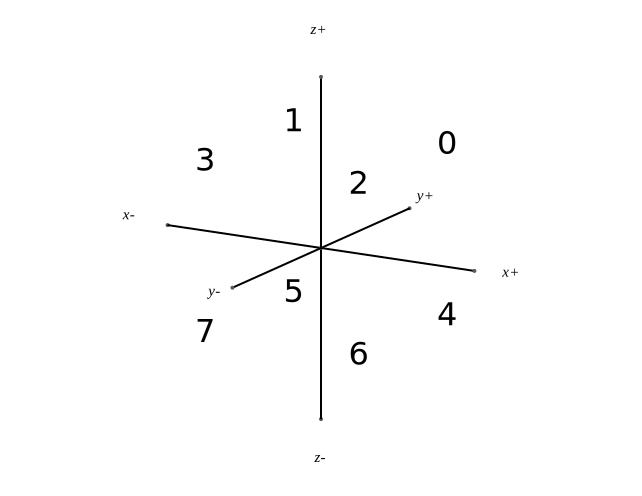
\includegraphics[width=0.7\linewidth]{esquemas/axes-with-octs}
 \end{center}
% \caption{\label{fig:nocts}Asignación de un índice~$n$ a cada octante de forma tal que el desarrollo binario de~$n$ indique los cambios de signos de los eje~$x$, $y$ y~$z$ con respecto al primer octante $n=0$.}
% \end{figure}
\end{minipage}

Notamos que el desarrollo binario del índice~$n$ tiene tres bits y éstos indican si hubo un cambio de signo o no en cada uno de los tres ejes con respecto al primer cuadrante, que corresponde a~$n=0$. De esta manera, podemos generar las direcciones~$\boldsymbol{\hat{\Omega}}_m$ para~$m=N(N+2)/8+1, N(N+2)$ a partir de las direcciones del primer cuadrante~$\boldsymbol{\hat{\Omega}}_j$ para~$j=1,N(N+2)/8$ con el algoritmo de la figura~\ref{alg:extension}, donde el símbolo ampersand~\texttt{\&} indica el operador binario \texttt{AND} y el signo de pregunta~\texttt{?} el operador ternario de decisión. La figura~\ref{fig:latsn} muestra el detalle de las latitudes y longitudes en la esfera unitaria del primer cuadrante y el conjunto resultante de las $N(N+2)$ direcciones para~S$_2$, S$_4$ y~$S_6$ que resultan de aplicar este desarrollo.

\begin{algorithm}
\DontPrintSemicolon
\For{$n = 1, \dots, 7$}{ 
 \For{$j = 1, \dots, N(N+2)/8$}{
  $\Omega_{n\cdot N(N+2)/8 + j \, , \, x} = ((n \& 1) ? (-1) : (+1)) \cdot \Omega_{j \, , \, x}$\;
  $\Omega_{n\cdot N(N+2)/8 + j \, , \, y} = ((n \& 2) ? (-1) : (+1)) \cdot \Omega_{j \, , \, y}$\;
  $\Omega_{n\cdot N(N+2)/8 + j \, , \, z} = ((n \& 4) ? (-1) : (+1)) \cdot \Omega_{j \, , \, z}$\;
  $w_{n\cdot N(N+2)/8 + j} = w_j$\;
  }
 }
\caption{\label{alg:extension}Extensión del primer octante a los otros siete}
\end{algorithm}

\begin{figure}[p]
\begin{center}
\subfloat[S$_2$]{%
\includegraphics[width=0.4\linewidth]{esquemas/lats2-nice}\hspace{2cm}
\includegraphics[width=0.3\linewidth]{esquemas/dirs2-nice}
}

\subfloat[S$_4$]{%
\includegraphics[width=0.4\linewidth]{esquemas/lats4-nice}\hspace{2cm}
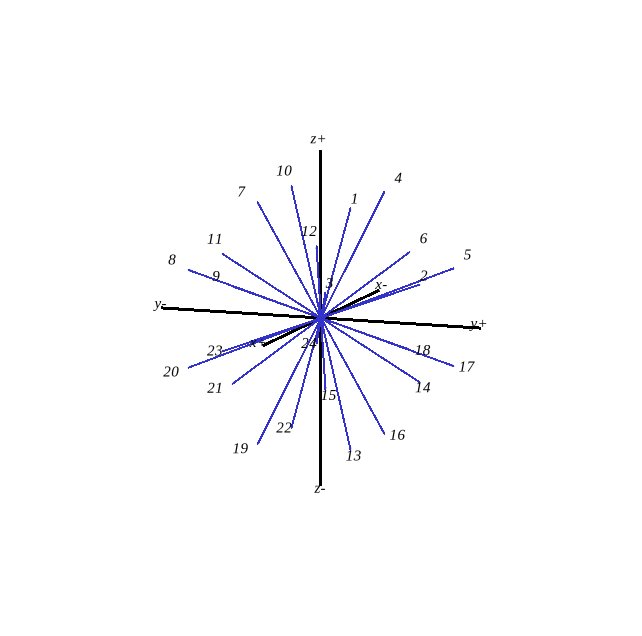
\includegraphics[width=0.3\linewidth]{esquemas/dirs4-nice}
}

 \subfloat[S$_6$]{%
\includegraphics[width=0.4\linewidth]{esquemas/lats6-nice}\hspace{2cm}
\includegraphics[width=0.3\linewidth]{esquemas/dirs6-nice}
}
\end{center}

\caption{\label{fig:latsn}Latitudes y longitudes en el primer cuadrante (izquierda) y conjunto de las~$N(N+2)$ direcciones de la cuadratura de nivel simétrico para~S$_2$, S$_4$ y~$S_6$ generadas a partir de un único coseno director positivo~$\mu_1$ de la tabla~\ref{tab:quadratureset}, aplicando con la ecuación~\eqref{eq:cosenos} para obtener el resto de los cosenos positivos, permutándolos según la tabla~\ref{tab:mus} y extendiéndolos al resto de los octantes con el algoritmo~\ref{alg:extension}. Las figuras son reproducciones tridimensionales realizadas con la herramienta Gmsh a partir de la información calculada y que realmente utiliza milonga (capítulo~\ref{cap:implementacion}) para realizar cálculos de transporte con el método de las ordenadas discretas.}
\end{figure}


\subsection{Dos dimensiones} % WIP
\label{sec:dosdimensiones}

El caso bidimensional en realidad es un problema en tres dimensiones pero sin dependencia de los parámetros del problema en una de las variables espaciales, digamos~$z$. De esta manera, el dominio~$U$ de la geometría está definido sólo sobre el plano~$x$-$y$ y las direcciones de vuelo~$\omegaversor$ de los neutrones son simétricas con respecto a este plano ya que por cada dirección~$\omegaversor = [\hat{\Omega}_x \, \hat{\Omega}_y \, \hat{\Omega}_z]$ con~$\hat{\Omega}_z>0$ hay una dirección simétrica~$\omegaprimaversor = [\hat{\Omega}_x \, \hat{\Omega}_y \, -\hat{\Omega}_z]$ (figura~\ref{fig:symmetry2d}). Luego, las posibles direcciones se reducen a la mitad, es decir~$N(N+2)/2$.

\begin{figure}
 \begin{center}
  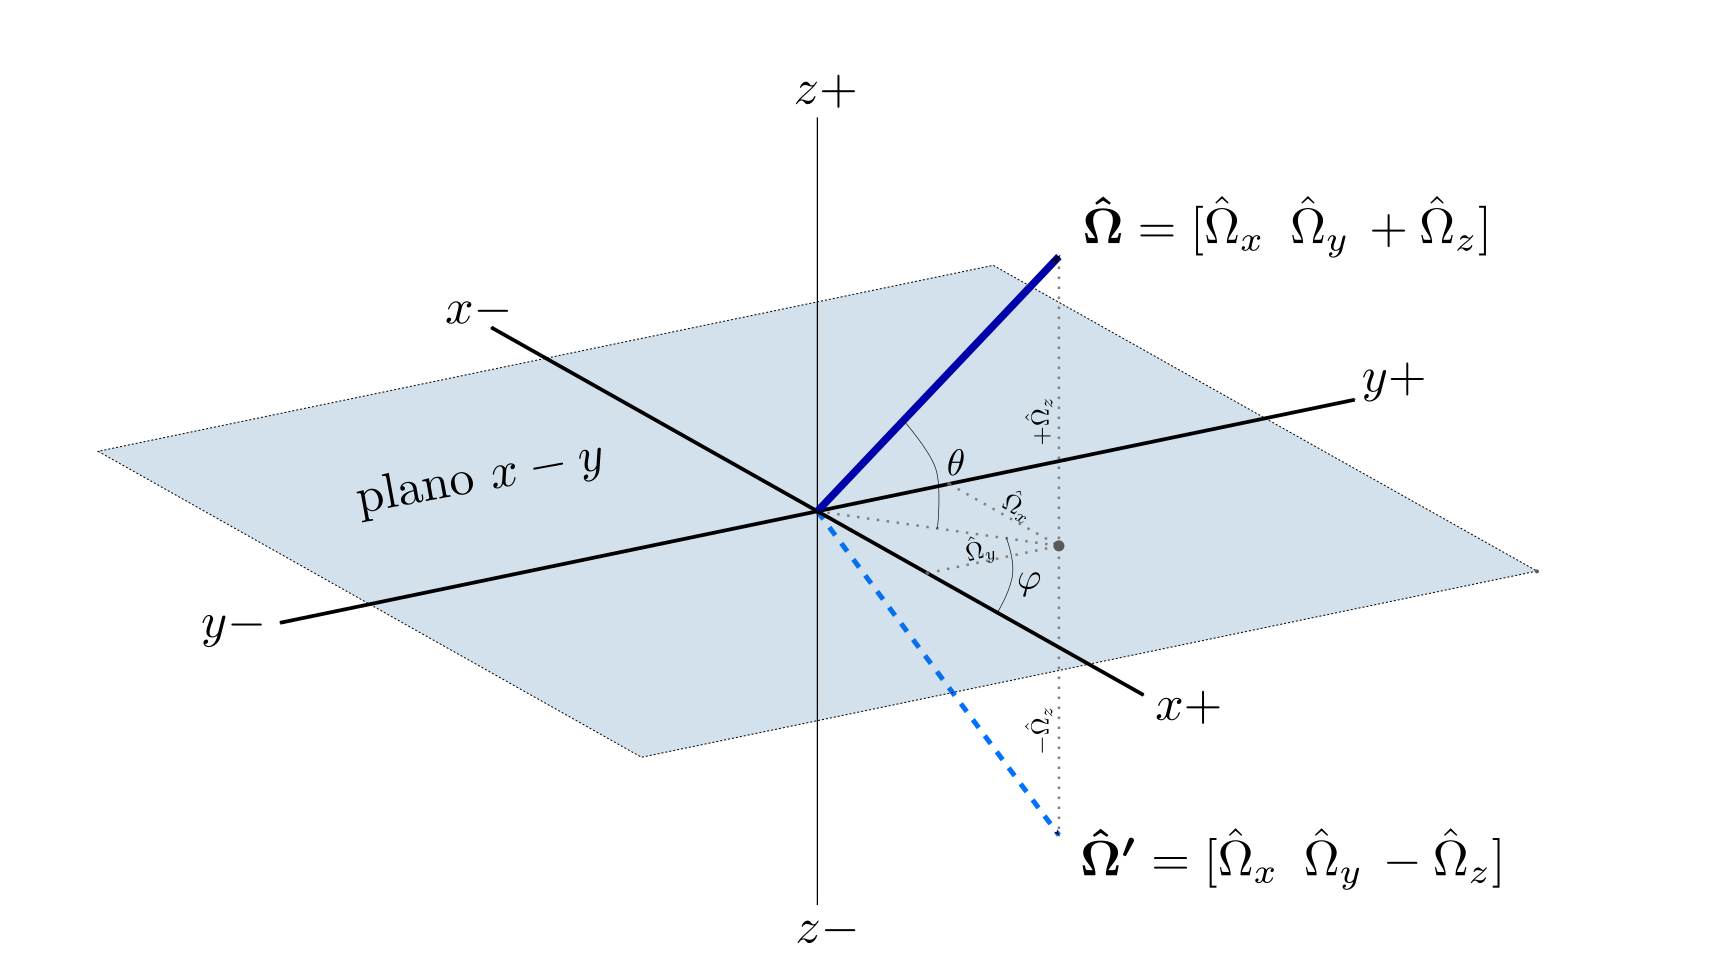
\includegraphics[scale=0.3]{esquemas/symmetry2d}
 \end{center}
\caption{\label{fig:symmetry2d}Simetría con respecto al plano~$x$-$y$ en un problema bi-dimensional. Por cada dirección~$\omegaversor$ con componente~$z$ positiva (línea llena) hay una dirección~$\omegaprimaversor$ simétrica e igualmente posible con~$\hat{\Omega}_z<0$ (línea de trazos).}
\end{figure}


Como la derivada espacial del flujo angular con respecto a~$z$ es cero entonces por un lado podemos escribir el término de transporte en la ecuación~\eqref{eq:transportesngeneral} como

\begin{equation*}
 \hat{\Omega}_{mx} \cdot \frac{\partial{\psi_{mg}}(x,y)}{\partial x} + \hat{\Omega}_{my} \cdot \frac{\partial{\psi_{mg}(x,y)}}{\partial y}
\end{equation*}
% 
donde ahora~$m=1,\dots,M = N(N+2)/2$. La componente~${\Omega}_{mz}$ no aparece explícitamente en las ecuaciones pero sí lo hace implícitamente en la elección de las direcciones, ya que siguen siendo válidas las ecuaciones~\eqref{eq:normalizaciondirecciones} y~\eqref{eq:normalizacionpesos}. Esto implica que en cada cuadrante tenemos nuevamente~$N(N+2)/8$ direcciones posibles, que luego debemos rotar para obtener las~$M$ direcciones en los cuatro cuadrantes. Dado que por un lado los pesos deben estar normalizados a uno y por otro para cada dirección con~$\hat{\Omega}_z>0$ hay otra dirección simétrica con~$\hat{\Omega}_z<0$, entonces el conjunto de cuadraturas de nivel simétrico para el primer cuadrante de un dominio de dos dimensiones consiste en las mismas~$N(N+2)/8$ direcciones correspondientes a tres dimensiones definidas en las tablas~\ref{tab:quadratureset} y~\ref{tab:mus}, cada una con el doble de peso. En forma equivalente, podemos concluir que las tablas~\ref{tab:quadratureset} y~\ref{tab:mus} valen para dos dimensiones con la salvedad de que el título de la tercera columna de la tabla~\ref{tab:quadratureset} debe ser~$4\cdot w_i$ en lugar de~$8\cdot w_i$ y debemos reemplazar la palabra “octante” por “cuadrante.” En la figura~\ref{fig:direcciones2d} mostramos las direcciones para la cuadratura de nivel simétrico utilizado en este trabajo para problemas de dos dimensiones espaciales. 

\begin{figure}
 \begin{center}
  \subfloat[S$_2$]{\includegraphics[scale=0.75]{esquemas/direcciones2ds2}}\\
  \subfloat[S$_4$]{\includegraphics[scale=0.75]{esquemas/direcciones2ds4}}\\
  \subfloat[S$_6$]{\includegraphics[scale=0.75]{esquemas/direcciones2ds6}}
 \end{center}
\caption{\label{fig:direcciones2d}Direcciones para el conjunto de cuadraturas de nivel simétrico en dos dimensiones.}
\end{figure}



\subsection{Una dimensión} % WIP

El caso unidimensional es radicalmente diferente a los otros dos. Si tomamos al eje~$x$ como la dirección de dependencia espacial, las posibles direcciones de viaje pueden depender sólo del ángulo cenital~$\theta$ ya que la simetría implica que todas las posibles direcciones azimutales con respecto al eje~$x$ son igualmente posibles.

\begin{figure}
 \begin{center}
  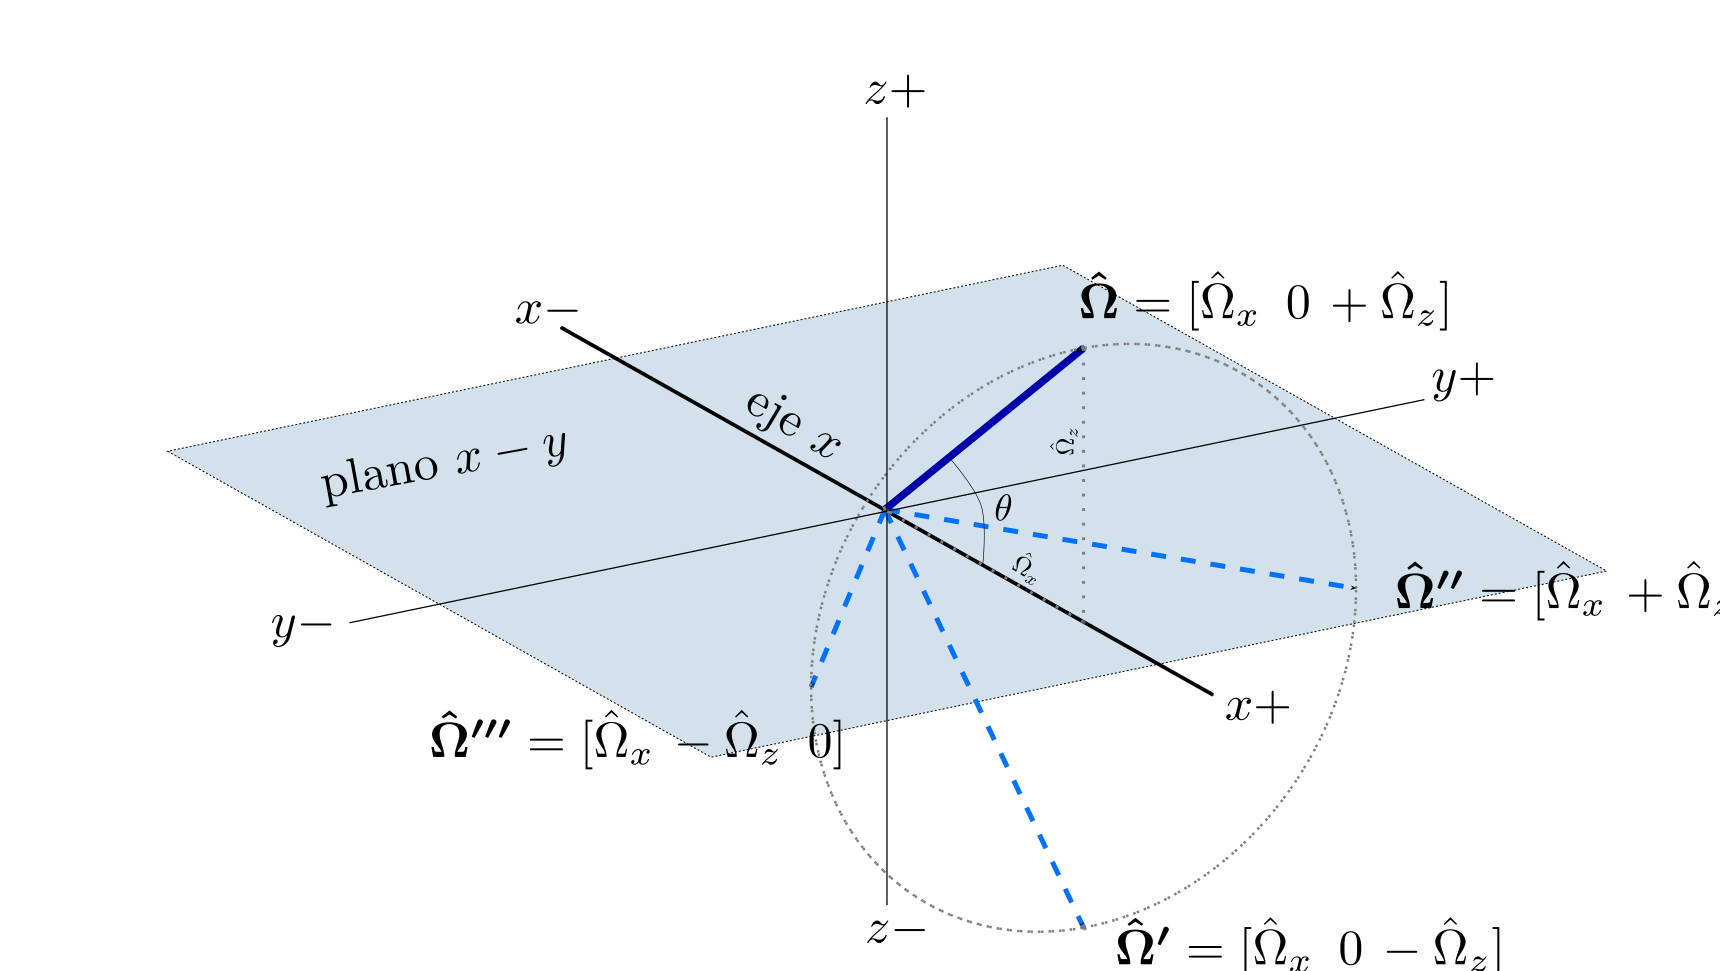
\includegraphics[scale=0.3]{esquemas/symmetry1d}
 \end{center}
\caption{\label{fig:symmetry1d}Simetría con respecto al eje~$x$ en un problema unidimensional. Por cada dirección~$\omegaversor$ (línea llena) hay infinitas direcciones simétricas e igualmente posibles apuntando en la dirección del círculo subtendido por el ángulo~$\theta=\arctan(\hat{\Omega}_z/\hat{\Omega}_x)$, representadas por las tres direcciones primadas (líneas de trazos).}
\end{figure}

El término de transporte de la ecuación~\eqref{eq:transportesngeneral} es entonces

\begin{equation*}
 \hat{\Omega}_{mx} \cdot \frac{\partial{\psi_{mg}}(x)}{\partial x} 
\end{equation*}

El hecho de que no una sino dos componentes de~$\omegaversor$ no aparezcan explícitamente relaja mucho más las condiciones para la elección de las~$M=N$ direcciones. En efecto, la única condición es simetría completa entre el semieje~$x>0$ y el semieje~$x<0$, lo que nos deja con~$N/2$ direcciones en cada semieje, todas ellas libres e independientes.

Para seleccionar las~$N/2$ direcciones y sus pesos asociados, notamos que en una dimensión

\begin{equation}\label{eq:1dgauss}
 \int_{4\pi} f(\omegaversor) \, d\omegaversor = 2\pi \int_{-1}^{1} f(\hat{\Omega}_x) \, d\hat{\Omega}_x \simeq 
2\pi \sum_{m=1}^N \omega_m \cdot f_m =
4\pi \sum_{m=1}^N \frac{\omega_m}{2} \cdot f_m =
4\pi \sum_{m=1}^N w_m \cdot f_m
\end{equation}

Si los puntos~$\hat{\Omega}_{xm}$ y los pesos~$\omega_m=2\cdot w_m$ son los asociados a la integración de Gauss y~$f(\hat{\Omega}_x)$ es un polinomio de orden~$2N-1$ o menos, entonces la integración es exacta (ver apéndice~\ref{sec:gauss}) y la ecuación~\eqref{eq:1dgauss} deja de ser una aproximación para transformarse en una igualdad. En la tabla~\ref{tab:gauss1d} mostramos el conjunto de cuadraturas utilizadas para una dimensión, que contiene esencialmente las abscisas y los pesos de la cuadratura de Gauss.

\begin{table}[t]
\begin{center}
%  \begin{tabularx}{0.4\linewidth}{cXcXc}
\begin{tabular}{cccc}
\hline
\hline
        & $m$ &  $\hat{\Omega}_{mx}$   & $\omega_m = 2 \cdot w_m$ \\
\hline              
  S$_2$ & 1   & $\sqrt{\frac{1}{3}}$   & 1   \\
                     
\hline              
  S$_4$ & 1   & $\sqrt{\frac{3}{7}-\frac{2}{7}\sqrt{\frac{6}{5}}}$ &    0.6521451549   \\
        & 2   & $\sqrt{\frac{3}{7}+\frac{2}{7}\sqrt{\frac{6}{5}}}$ &    0.3478548451   \\

\hline              
  S$_6$ & 1     & 0.2386191860   & 0.4679139346   \\
        & 2     & 0.6612093864   & 0.3607615730   \\
        & 3     & 0.9324695142   & 0.1713244924   \\

\hline              
  S$_8$ & 1     & 0.1834346424  & 0.3626837834   \\
        & 2     & 0.5255324099  & 0.5255324099    \\
        & 3     & 0.7966664774  & 0.2223810344   \\
        & 4     & 0.9602898564  & 0.1012285363   \\
\hline
\hline
\end{tabular}
\end{center}
\caption{\label{tab:gauss1d}Conjuntos de cuadratura para problemas unidimensionales. Las direcciones~$\hat{\Omega}_{mx}$ coinciden con las abscisas de la cuadratura de Gauss. Los pesos~$w_m$ de ordenadas discretas son la mitad de los pesos~$\omega_m$ de la cuadratura de Gauss. Las direcciones~$m=N/2+1,\dots,N$ no se muestran pero se obtienen como~$\hat{\Omega}_{N/2+m \, x} = -\hat{\Omega}_{mx}$ y~$w_{N/2+m} = w_m$.}
\end{table}

\section{Formulaciones fuertes, integrales y débiles} % WIP

Antes de comenzar a discutir las discretizaciones espaciales tanto de la ecuación de transporte multigrupo con ordenadas discretas como de la ecuación de difusión multigrupo, introducimos las ideas de formulaciones fuertes, integrales y débiles sobre las que se basan los esquemas de discretización numérica basados en diferencias finitas, en volúmenes finitos y en elementos finitos respectivamente. De esta forma, además, resumimos las ecuaciones en derivadas parciales con respecto a las coordenadas espaciales que debemos resolver para obtener la distribución de flujo neutrónico de estado estacionario en un reactor nuclear.

\subsection{Formulaciones fuertes} % WIP
\label{sec:fuertes}

La formulación fuerte de un problema de derivadas parciales consiste en escribir directamente las ecuaciones diferenciales y sus condiciones de contorno. Más específicamente:

\begin{definicion}
 Decimos que un problema en derivadas parciales está escrito en su formulación fuerte cuando en el sistema de ecuaciones diferenciales y sus condiciones de contorno el orden de las derivadas es igual al orden del problema. Es decir, en la formulación fuerte no hay operadores integrales que no son esenciales para la definición del problema.
\end{definicion}

Hasta este momento, en esta tesis hemos escrito ecuaciones diferenciales que son la formulación fuerte tanto del problema de transporte como del problema de difusión de neutrones. Si bien matemáticamente el desarrollo fue lógico y correcto, hay salvedades que tenemos que notar. Por ejemplo, el término de fugas de la ecuación de difusión de neutrones multigrupo~\eqref{eq:difusionmultigrupo} es

\begin{equation*}
 - \text{div} \Big[ D_g(\vec{x}) \cdot \text{grad} \left[ \phi_g(\vec{x}) \right] \Big]
\end{equation*}

Si el coeficiente de difusión~$D_g$ presenta una discontinuidad en~$\vec{x}$, por ejemplo debido a que hay una interfaz entre dos materiales diferentes, entonces este término no está definido y no puede ser evaluado. Este es uno de los varios inconvenientes que tiene esta formulación a la hora de utilizarla para resolver numéricamente los problemas planteados en esta tesis. 

\subsubsection{Ordenadas discretas} % WIP

La formulación fuerte del problema de transporte de neutrones discretizado en energía mediante el método multigrupo y en ángulo mediante ordenadas discretas es la ecuación diferencial~\eqref{eq:transportesngeneral}

\begin{multline}\tag{\ref{eq:transportesngeneral}}
 \omegaversor_m \cdot \text{grad} \left[ \psi_{mg}(\vec{x}) \right]
 + \Sigma_{t g}(\vec{x}) \cdot \psi_{mg}(\vec{x}) = \\
  \sum_{g^\prime=1}^G \sum_{m^\prime=1}^M w_{m^\prime} \cdot
\left[  \sum_{\ell=0}^\infty (2\ell+1) \cdot \Sigma_{s_\ell \,g^\prime \rightarrow g}(\vec{x}) \cdot P_\ell (\omegaversor_m \cdot \boldsymbol{\hat{\Omega}^\prime}_{m^\prime}) \right]
 \cdot \psi_{m^\prime g^\prime}(\vec{x}) \\
+ \chi_g \sum_{g^\prime=1}^G \nu\Sigma_{fg^\prime}(\vec{x}) \sum_{m^\prime=1}^M w_{m^\prime} \cdot \psi_{m^\prime g^\prime}(\vec{x})
+ s_{mg}(\vec{x})
\end{multline}
%
sobre el dominio espacial~$U \in \mathbb{R}^n$ ($n=1,2,3$) para el grupo de energía~$g=1,\dots,G$ y para la dirección~$m=1,\dots,M$ con las condiciones de contorno de Dirichlet discutidas en la sección~\ref{sec:bctransporte}:

\begin{equation}\label{eq:transportesncc}
\psi_{mg}^{ij} =
 \begin{cases}
  \psi_{mg}(\vec{x}) = 0 
&\quad\quad \forall \vec{x} \in \Gamma_V \wedge \omegaversor_m \cdot \hat{\vec{n}}(\vec{x}) < 0 \\
  \psi_{mg}(\vec{x}) = \psi_{mg^\prime} \quad / \quad \omegaversor_{g^\prime} = \omegaversor_m - 2 \left( \omegaversor_m \cdot \hat{\vec{n}} \right) \hat{\vec{n}}
&\quad\quad \forall \vec{x} \in \Gamma_M \wedge \omegaversor_m \cdot \hat{\vec{n}}(\vec{x}) < 0 \\
  \psi_{mg}(\vec{x}) = f_{mg}(\vec{x})
&\quad\quad \forall \vec{x} \notin \Gamma_V \bigcup \Gamma_M \wedge \omegaversor_m \cdot \hat{\vec{n}}(\vec{x}) < 0 \\
 \end{cases}
\end{equation}

Si el término de fuentes independientes~$s_{mg}$ en la ecuación~\eqref{eq:transportesngeneral} es nulo, entonces las condiciones de contorno deben ser homogénes, es decir~$\Gamma_V \bigcup \Gamma_M = \partial U$ (recordar las deficiones~\ref{def:ccvacuum} y~\ref{def:ccmirror}). Además debemos incluir el factor de multiplicación efectivo~$k_\text{eff}$ dividiendo al término de fisiones de la ecuación~\eqref{eq:transportesngeneral}:

\begin{multline}\label{eq:transportesnkeff}
 \omegaversor_m \cdot \text{grad} \left[ \psi_{mg}(\vec{x}) \right]
 + \Sigma_{t g}(\vec{x}) \cdot \psi_{mg}(\vec{x}) = \\
  \sum_{g^\prime=1}^G \sum_{m^\prime=1}^M w_{m^\prime} \cdot
\left[  \sum_{\ell=0}^\infty (2\ell+1) \cdot \Sigma_{s_\ell \,g^\prime \rightarrow g}(\vec{x}) \cdot P_\ell (\omegaversor_m \cdot \boldsymbol{\hat{\Omega}^\prime}_{m^\prime}) \right]
 \cdot \psi_{m^\prime g^\prime}(\vec{x}) \\
+ \frac{\chi_g}{k_\text{eff}} \sum_{g^\prime=1}^G \nu\Sigma_{fg^\prime}(\vec{x}) \sum_{m^\prime=1}^M w_{m^\prime} \cdot \psi_{m^\prime g^\prime}(\vec{x})
\end{multline}

\subsubsection{Difusión} % WIP

La formulación fuerte del problema de difusión de neutrones discretizado en energía mediante el método multigrupo es la ecuación~\eqref{eq:difusionmultigrupo}

\begin{multline}\tag{\ref{eq:difusionmultigrupo}}
 - \text{div} \Big[ D_g(\vec{x}) \cdot \text{grad} \left[ \phi_g(\vec{x}) \right] \Big]
 + \Sigma_{t g}(\vec{x}) \cdot \phi_g(\vec{x})
 = \\
\sum_{g^\prime = 1}^G \Sigma_{s_0 g^\prime \rightarrow g}(\vec{x})  \cdot \phi_{g^\prime}(\vec{x}) +
\chi_g \sum_{g^\prime = 1}^G \nu\Sigma_{fg^\prime}(\vec{x}) \cdot \phi_{g^\prime}(\vec{x})+ s_{0_g}(\vec{x})
\end{multline}
%
sobre el dominio espacial~$U \in \mathbb{R}^n$ ($n=1,2,3$) para el grupo de energía~$g=1,\dots,G$ con las condiciones de contorno discutidas en la sección~\ref{sec:bcdifusion}:

\begin{equation}\label{eq:difusioncc}
 \begin{cases}
  \phi_g(\vec{x}) = 0 
&\quad\quad \forall \vec{x} \in \Gamma_N \\
  \displaystyle \frac{\partial \phi_g}{\partial n} = 0
&\quad\quad \forall \vec{x} \in \Gamma_M \\
  \phi_g(\vec{x}) + 2\cdot D_g(\vec{x}) \cdot \displaystyle \frac{\partial \phi_g}{\partial n} = 0
&\quad\quad \forall \vec{x} \in \Gamma_V \\
  a_g(\vec{x} \cdot \phi_g(\vec{x}) + b_g(\vec{x}) \cdot \displaystyle \frac{\partial \phi_g}{\partial n} = c_g(\vec{x}
&\quad\quad \forall \vec{x} \notin \Gamma_N \bigcup \Gamma_M \bigcup \Gamma_V \\
 \end{cases}
\end{equation}

Nuevamente, si el término de fuentes independientes~$s_{0g}$ es nulo entonces las condiciones de contorno deben ser homogéneas, i.e.~$\Gamma_N \bigcup \Gamma_M \bigcup \Gamma_V = \partial U$ (definiciones~\ref{def:ccvacuumdif}, \ref{def:ccmirrordif} y~\ref{def:ccnulldif}). Además debemos dividir el término de fuentes por el factor de multiplicación efectivo~$k_\text{eff}$:

\begin{multline}\label{eq:difusionmultigrupokeff}
 - \text{div} \Big[ D_g(\vec{x}) \cdot \text{grad} \left[ \phi_g(\vec{x}) \right] \Big]
 + \Sigma_{t g}(\vec{x}) \cdot \phi_g(\vec{x})
 = \\
\sum_{g^\prime = 1}^G \Sigma_{s_0 g^\prime \rightarrow g}(\vec{x})  \cdot \phi_{g^\prime}(\vec{x}) +
\frac{\chi_g}{k_\text{eff}} \sum_{g^\prime = 1}^G \nu\Sigma_{fg^\prime}(\vec{x}) \cdot \phi_{g^\prime}(\vec{x})
\end{multline}

\subsection{Formulaciones integrales} % WIP
\label{sec:integrales}

Dado que las ecuaciones de la sección anterior se cumplen punto a punto, podemos operar lógica y matemáticamente sobre ellas para obtener otras formulaciones más adecuadas para ser atacadas por esquemas de discretización espacial. Las formulaciones integrales son la base de los métodos basdos en volúmenes finitos y consisten en integrar las ecuaciones sobre volúmenes de control. 

\subsubsection{Ordenadas discretas} % WIP

Tomemos la ecuación~\eqref{eq:transportesngeneral} e integrémosla en un cierto volumen~$V \subset U \subset \mathbb{R}^n$:

\begin{multline*}
 \int_V \omegaversor_m \cdot \text{grad} \left[ \psi_{mg}(\vec{x}) \right] \, d^n\vec{x}
 +
 \int_V \Sigma_{t g}(\vec{x}) \cdot \psi_{mg}(\vec{x}) \, d^n\vec{x} = \\
 \bigintsss_V \sum_{g^\prime=1}^G \sum_{m^\prime=1}^M w_{m^\prime} \cdot
\left[  \sum_{\ell=0}^\infty (2\ell+1) \cdot \Sigma_{s_\ell \,g^\prime \rightarrow g}(\vec{x}) \cdot P_\ell (\omegaversor_m \cdot \boldsymbol{\hat{\Omega}^\prime}_{m^\prime}) \right]
 \cdot \psi_{m^\prime g^\prime}(\vec{x}) \, d^n\vec{x} \\
+
 \int_V \chi_g \sum_{g^\prime=1}^G \nu\Sigma_{fg^\prime}(\vec{x}) \sum_{m^\prime=1}^M w_{m^\prime} \cdot \psi_{m^\prime g^\prime}(\vec{x}) \, d^n\vec{x}
+
 \int_V s_{mg}(\vec{x}) \, d^n\vec{x}
\end{multline*}

Dado que~$\omegaversor_m$ no depende de~$\vec{x}$, podemos evaluar el primer término como

\begin{align*}
 \int_V \omegaversor_m \cdot \text{grad} \left[ \psi_{mg}(\vec{x}) \right] \, d^n\vec{x} &=
 \int_V \text{div} \left[ \omegaversor_m \cdot \psi_{mg}(\vec{x}) \right] \, d^n\vec{x} \\
&=
 \int_S \left[ \omegaversor_m \cdot \psi_{mg}(\vec{x}) \right] \cdot \hat{\vec{n}}(\vec{x}) \, d^{n-1}\vec{x} \\
&=
 \int_S \psi_{mg}(\vec{x}) \cdot \left[ \omegaversor_m \cdot \hat{\vec{n}}(\vec{x})\right]  \, d^{n-1}\vec{x}
\end{align*}
%
donde hemos utilizado el teorema de la divergencia, $S$ es la superficie del volúmen~$V$ y~$\hat{\vec{n}}$ es el versor normal a la superficie~$S$ en el punto~$\vec{x}$ orientado hacia la dirección exterior al volumen~$V$. Es justamente esta operación, que reduce en uno el orden del operador diferencia, la que hace que la formulación integral sea de utilidad para la discretización espacial. De hecho en el caso de la ecuación de transporte, este operador diferencial se transforma en algebraico. En cualquier caso, la formulación integral de la ecuación de transporte con ordenadas discretas es


\begin{multline}\label{eq:transportesnintegral}
 \int_S \psi_{mg}(\vec{x}) \cdot \left[ \omegaversor_m \cdot \hat{\vec{n}}(\vec{x})\right]  \, d^{n-1}\vec{x}
 +
 \int_V \Sigma_{t g}(\vec{x}) \cdot \psi_{mg}(\vec{x}) \, d^n\vec{x} = \\
 \sum_{g^\prime=1}^G \sum_{m^\prime=1}^M  w_{m^\prime} \cdot  \sum_{\ell=0}^\infty 
\int_V \Sigma_{s_\ell \,g^\prime \rightarrow g}(\vec{x}) \cdot (2\ell+1) \cdot P_\ell (\omegaversor_m \cdot \boldsymbol{\hat{\Omega}^\prime}_{m^\prime}) \cdot \psi_{m^\prime g^\prime}(\vec{x}) \, d^n\vec{x} \\
+
 \chi_g  \sum_{g^\prime=1}^G \sum_{m^\prime=1}^M  w_{m^\prime} \cdot \int_V \nu\Sigma_{fg^\prime}(\vec{x}) \cdot \psi_{m^\prime g^\prime}(\vec{x}) \, d^n\vec{x}
+
 \int_V s_{mg}(\vec{x}) \, d^n\vec{x}
\end{multline}
%
sobre el dominio espacial~$U \in \mathbb{R}^n$ ($n=1,2,3$) para el grupo de energía~$g=1,\dots,G$ con las mismas condiciones de contorno de la formulación fuerte de la ecuación~\eqref{eq:transportesncc}. Debemos notar que un conjunto de funciones solución~$\psi_{mg}$ que satisfaga la formulación débil entonces también va a satisfacer la formulación integral. Sin embargo, podemos encontrar otro conjunto de funciones solución~$\psi_{mg}^\prime$ que satisfaga la formulación integral pero que no satisfaga la formulación débil. De hecho, justamente las soluciones encontradas con el método de volúmenes finitos satisfacen la formulación integral pero no la formulación débil para volúmenes de control~$V$ de tamaño finito.

\subsubsection{Difusión} % WIP

Procediendo en forma análoga, integramos la formulación fuerte~\eqref{eq:difusionmultigrupo} sobre un volúmen de control~$V \subset U \subset \mathbb{R}^n$:

\begin{multline*}
 - \int_V \text{div} \Big[ D_g(\vec{x}) \cdot \text{grad} \left[ \phi_g(\vec{x}) \right] \Big] \, d^n \vec{x}
 + \int_V \Sigma_{t g}(\vec{x}) \cdot \phi_g(\vec{x}) \, d^n \vec{x}
 = \\
 \int_V \sum_{g^\prime = 1}^G \Sigma_{s_0 g^\prime \rightarrow g}(\vec{x})  \cdot \phi_{g^\prime}(\vec{x}) \, d^n \vec{x}
+
 \int_V \chi_g \sum_{g^\prime = 1}^G \nu\Sigma_{fg^\prime}(\vec{x}) \cdot \phi_{g^\prime}(\vec{x}) \, d^n \vec{x}
 +
\int_V s_{0_g}(\vec{x}) \, d^n \vec{x}
\end{multline*}
%
sobre el dominio espacial~$U \in \mathbb{R}^n$ ($n=1,2,3$) para el grupo de energía~$g=1,\dots,G$. Aplicando nuevamente el teorema de la divergencia al primer término, tenemos

\begin{equation*}
\int_V \text{div} \Big[ D_g(\vec{x}) \cdot \text{grad} \left[ \phi_g(\vec{x}) \right] \Big] \, d^n \vec{x} =
\int_S D_g(\vec{x}) \cdot \Big[ \text{grad} \left[ \phi_g(\vec{x}) \right] \cdot \hat{\vec{n}}(\vec{x}) \Big] \, d^{n-1} \vec{x}
\end{equation*}
%
donde nuevamente~$S$ es la superficie del volúmen~$V$ y~$\hat{\vec{n}}$ es el versor normal exterior a la superficie~$S$. De esta manera hemos reducido el orden de la ecuación de dos a uno para obtener la formulación integral como

\begin{multline}\label{eq:difusionintegral}
 - \int_S D_g(\vec{x}) \cdot \Big[ \text{grad} \left[ \phi_g(\vec{x}) \right] \cdot \hat{\vec{n}}(\vec{x}) \Big] \, d^{n-1} \vec{x}
 + \int_V \Sigma_{t g}(\vec{x}) \cdot \phi_g(\vec{x}) \, d^n \vec{x}
 = \\
 \sum_{g^\prime = 1}^G \int_V \Sigma_{s_0 g^\prime \rightarrow g}(\vec{x})  \cdot \phi_{g^\prime}(\vec{x}) \, d^n \vec{x}
+
 \chi_g \sum_{g^\prime = 1}^G \int_V  \nu\Sigma_{fg^\prime}(\vec{x}) \cdot \phi_{g^\prime}(\vec{x}) \, d^n \vec{x}
 +
\int_V s_{0_g}(\vec{x}) \, d^n \vec{x}
\end{multline}
%
con las condiciones de contorno descriptas en la ecuación~\eqref{eq:difusioncc}.

\subsection{Formulaciones débiles} % TBD
\label{sec:debiles}

{\color{red}TO BE DONE}

\subsubsection{Ordenadas discretas} % TBD

{\color{red}TO BE DONE}

\subsubsection{Difusión} % TBD

{\color{red}TO BE DONE}

\section{Discretización espacial} % WIP
\label{sec:discretizacion_espacial}
El objetivo de la discretización espacial es obtener a partir de ecuaciones que sólo dependen de la coordenada espacial~$\vec{x}$ un sistema de ecuaciones algebraicas cuyas incógnitas sean los valores que toma el flujo ($\psi$ angular para transporte y escalar~$\phi$ para difusión) en una cierta cantidad~$T$ finita de puntos del espacio: el centro de las celdas para volúmenes finitos y los nodos para elementos finitos, como mostramos a continuación. Para simplificar la notación, utilizamos el concepto de \emph{vector incógnita}.

\begin{definicion}
Sea~$\boldsymbol{\xi} \in \mathbb{R}^{TGM}$ un vector cuyos elementos son los flujos incógnita~$\psi_{mg}^t$ para las~$m=1,\dots,M$ direcciones discretas, los~$g=1,\dots,G$ grupos de energía evaluado en los~$t=1,\dots,T$ puntos~$\vec{x}_t$ del espacio, ordenados de alguna cierta manera. Para el caso de difusión tomamos~$M=1$ y~$\psi_{1g}^t = \phi_{g}^t$. Llamamos a~$\boldsymbol{\xi}$ el \emph{vector incógnita}. 
\end{definicion}

Si las secciones eficaces sólo dependen de la posición~$\vec{x}$ y no del nivel de flujo de neutrones, entonces la ecuación de transporte---y por lo tanto también la de difusión---es lineal sobre el flujo. Como demostramos en lo que resta del capítulo, resulta entonces que la formulación del problema discretizado puede ser escrita en forma matricial.

\begin{definicion}
Sean~$R$ y~$F$ son matrices de tamaño~$TGM \times TGM$ y $\vec{S}$ un vector de tamaño~$IGM$. Llamamos \emph{matriz de remoción} a~$R$, \emph{matriz de fisión} a~$F$ y \emph{vector de fuentes} a~$\vec{S}$. Los elementos de estos objetos dependen de la formulación (ordenadas discretas o difusión) y del esquema de discretización espacial (volúmenes o elementos finitos). 
\end{definicion}

Tenemos entonces dos casos que conducen a problemas matemáticos diferentes. El primero consiste en aquellos problemas en los que la fuente independiente~$s$ es diferente de cero en el dominio (multiplicativo o no), o bien en los que las condiciones de contorno son no homogéneas (por ejemplo debido a una corriente entrante no nula). El segundo es el caso de fuente independiente idénticamente nula y condiciones de contorno homogéneas en presencia de un medio multiplicativo. Este caso recibe el nombre de \emph{cálculo de criticidad}, donde además de una distribución espacial de flujo obtenemos un escalar que indica qué tan lejos de la criticidad está la geometría propuesta. En este trabajo utilizamos el concepto de \emph{reactor crítico asociado en~$k$}~\cite{duderstadt,henry} en el cual dividimos a los términos de fisión por un escalar~$k_\text{eff}$. Matemáticamente, veremos más adelante en este capítulo que podemos escribir  

\begin{itemize}
 \item Problema con fuente independiente no nula o con condiciones de contorno no homogéneas:
 
\begin{align*}
 R \cdot \boldsymbol{\xi} = F \cdot \boldsymbol{\xi} + \vec{S} \\
 (R-F) \cdot \boldsymbol{\xi} = \vec{S} \\
\end{align*}
 
 \item Problema sin fuente independiente con condiciones de contorno homogéneas:
 
\begin{align*}
 R \cdot \boldsymbol{\xi} = \frac{1}{k_\text{eff}} F \cdot \boldsymbol{\xi} \\
 k_\text{eff} \cdot R \cdot \boldsymbol{\xi} = F \cdot \boldsymbol{\xi} \\
\end{align*}
\end{itemize}



\subsection{Mallas estructuradas y no estructuradas} % TBD

cuatro figuras: un cuadrado uniforme, un cuadrado con deltas x e y no uniformes, un circulo con cosas radiales y un paralelogramo o algo curvo con elementos que se van curvando. El último es estructurado pero conviene tratarlo como no estructurado.

lo mismo no estructurado pero sobre algo que no sea un cuadrado (un cuadrado con un pedazo redondo?): es una generalización, el estrucutrado está contenido en el no estructurado.

ilustrar el efecto staircase, cuando realmente los elementos combustibles son cuadrados zafa, pero el reflector radial siempre es cilíndrico.

Definición de nodo: lo que tiene dimensión cero
Definición de celda: lo que tiene dimensión igual a la del problema

Todo lo demás, incluyendo nodos y celdas son elementos.

figuras de dmplex?

\lipsum[4]


\section{Volúmenes finitos} % WIP

El método de volúmenes finitos se basa en la formulación integral discutida en la sección~\ref{sec:integrales}. Los términos integrados sobre volúmenes son aproximados por un valor medio del integrando multiplicado por el volúmen de la celda. Los términos integrados sobre superficies son reemplazados por aproximaciones de los integrandos sobre las superficies a partir de los valores medios de las celdas adyacentes. Estos esquemas se basan más en un enfoque geométrico que en un formalismo matemático (al contrario de lo que sucede con el método de elementos finitos que discutimos en la sección~\ref{sec:elementos}), aunque es posible estudiar su errores y sus propiedades de convergencia~\cite{bookevol}.


\subsection{Ordenadas discretas en volúmenes} % WIP

En el método de los volúmenes finitos que proponemos, las incógnitas del problema son los valores medios de los flujos en las~$I$ celdas, a diferencia de lo que sucede en diferencias o elementos finitos donde las incógnitas son los valores que toman los flujos sobre los~$K$ nodos.

\begin{definicion}
El flujo angular del grupo~$g=1,\dots,G$ en la dirección~$m=1,\dots,M$ en la celda~$i=1,\dots,I$ es

\begin{equation}\label{eq:flujo-medio}
 \psi_{mg}^i = \frac{\displaystyle \int_{V_i} \psi_{mg}(\vec{x}) \, d^n\vec{x}}{\displaystyle \int_{V_i} \, d^n\vec{x}}
\end{equation}
%
donde~$V_i \in \mathbb{R}^n$ es el volumen del dominio~$U$ ocupado por la  celda~$i$.
\end{definicion}


De esta manera, el problema consiste en encontrar los~$I \cdot G \cdot M$ valores~$\psi_{mg}^i$, que son los elementos del vector incógnita~$\boldsymbol{\xi} \in \mathbb{R}^{IGM}$ definido en la ecuación~\eqref{eq:incognita}. Para ello, tomamos la formulación integral del problema de ordenadas discretas dada por la ecuación~\eqref{eq:transportesnintegral} introducida en la sección~\ref{sec:integrales}

\begin{multline}\tag{\ref{eq:transportesnintegral}}
 \int_S \psi_{mg}(\vec{x}) \cdot \left[ \omegaversor_m \cdot \hat{\vec{n}}(\vec{x})\right]  \, d^{n-1}\vec{x}
 +
 \int_V \Sigma_{t g}(\vec{x}) \cdot \psi_{mg}(\vec{x}) \, d^n\vec{x} = \\
 \sum_{g^\prime=1}^G \sum_{m^\prime=1}^M  w_{m^\prime} \cdot  \sum_{\ell=0}^\infty 
\int_V \Sigma_{s_\ell \,g^\prime \rightarrow g}(\vec{x}) \cdot (2\ell+1) \cdot P_\ell (\omegaversor_m \cdot \boldsymbol{\hat{\Omega}^\prime}_{m^\prime}) \cdot \psi_{m^\prime g^\prime}(\vec{x}) \, d^n\vec{x} \\
+
 \chi_g  \sum_{g^\prime=1}^G \sum_{m^\prime=1}^M  w_{m^\prime} \cdot \int_V \nu\Sigma_{fg^\prime}(\vec{x}) \cdot \psi_{m^\prime g^\prime}(\vec{x}) \, d^n\vec{x}
+
 \int_V s_{mg}(\vec{x}) \, d^n\vec{x}
\end{multline}
%
y analizamos cómo podemos aproximar cada término en función de las incógnitas del problema, que son los flujos medios el las celdas dados por la ecuación~\eqref{eq:flujo-medio}.

\subsubsection{Términos volumétricos} % WIP

Exceptuando el primer y el último término de la ecuación~\eqref{eq:transportesnintegral}, todos los demás tienen la forma

\begin{equation}\label{eq:snvol1}
\int_{V} f(\vec{x}) \cdot \psi_{mg}(\vec{x}) \, d^n\vec{x}
\end{equation}

Como la ecuación~\eqref{eq:transportesnintegral} vale para cualquier volumen~$V$ arbitrario, entonces deberá valer para cada volumen~$V_i$ de las~$I$ celdas que aproximan el dominio~$U \in \mathbb{R}^n$. En particular, podemos evaluar la ecuación~\eqref{eq:snvol1} para la celda~$i$-ésima  multiplicando y dividiendo por~$\int_{V_i} \, d^n\vec{x}$ y por~$\int_{V_i} \psi_{mg}(\vec{x}) d^n\vec{x}$ y recordando la definición~\eqref{eq:flujo-medio} de~$\psi_{mg}^i$

\begin{align}\label{eq:snvol2}
\int_{V_i} f(\vec{x}) \cdot \psi_{mg}(\vec{x}) \, d^n\vec{x} &=
\int_{V_i} f(\vec{x}) \cdot \psi_{mg}(\vec{x}) \, d^n\vec{x} \cdot
\frac{\displaystyle \int_{V_i} \, d^n\vec{x}}{\displaystyle \int_{V_i} \, d^n\vec{x}} \cdot
\frac{\displaystyle \int_{V_i} \psi_{mg}(\vec{x}) \, d^n\vec{x}}{\displaystyle \int_{V_i} \psi_{mg}(\vec{x}) \, d^n\vec{x}} \nonumber \\
&=
\frac{\displaystyle \int_{V_i} f(\vec{x}) \cdot \psi_{mg}(\vec{x}) \, d^n\vec{x}}{\displaystyle \int_{V_i} \psi_{mg}(\vec{x}) \, d^n\vec{x}} \cdot
\int_{V_i} \, d^n\vec{x} \cdot \psi_{mg}^i
\end{align}

Podemos aproximar la ecuación~\eqref{eq:snvol2} como

\begin{equation}\label{eq:snvol3}
  \int_{V_i} f(\vec{x}) \cdot \psi_{mg}(\vec{x}) \, d^n\vec{x} \approx
  \left[ \int_{V_i} f(\vec{x}) \, d^n\vec{x} \right] \cdot \psi_{mg}^i
=
 f^i \cdot V_i \cdot \psi_{mg}^i
\end{equation}
%
donde directamente denotamos con la variable~$V_i$ al volumen~$\int_{V_i} \, d^n\vec{x}$ de la celda.
Si~$f(\vec{x})$ es idénticamente igual a una constante $f^i$ para todo~$\vec{x} \in V_i$, entonces debemos reemplazar el signo de aproximación de la ecuación~\eqref{eq:snvol3} por un signo de igualdad. Si~$f(\vec{x})$ no es uniforme dentro de la celda~$i$, entonces debemos utilizar nuestro juicio de ingeniería para evaluar qué tan válida es esta aproximación en función del tamaño~$V_i$ de la celda y de la magnitud del cambio de~$f(\vec{x}$) dentro de la misma.

\subsubsection{Término de fugas} % WIP
\label{sec:snvolfugas}

Por otro lado, el primer término de la formulación integral~\eqref{eq:transportesnintegral} es el término que da la tasa neta de fugas a través de la superficie externa del volumen~$V$. En particular, para la celda~$i$, tenemos

\begin{equation*}
 \int_{S_i} \psi_{mg}(\vec{x}) \cdot \left[ \omegaversor_m \cdot \hat{\vec{n}}(\vec{x})\right]  \, d^{n-1}\vec{x}
= \sum_{j~\text{vecinos}} \int_{S_{ij}} \psi_{mg}(\vec{x}) \cdot \left( \omegaversor_m \cdot \hat{\vec{n}}_{ij}\right)  \, d^{n-1}\vec{x}
\end{equation*}
%
donde~$J$ es la cantidad de caras planas que definen a la celda~$i$ y~$S_{ij}$ es la superficie que separa a la celda~$i$ de la celda~$j$ adyacente. En este caso, $\hat{\vec{n}}_{ij}$ es el versor normal a la superficie~$S_{ij}$ en la dirección externa a la celda~$i$ (figura~\ref{fig:nij}). Decimos que las celdas~$i$ y~$j$ son \emph{vecinos}. Como las superficies son planas, entonces~$\hat{\vec{n}}_{ij}$ no depende de~$\vec{x}$ y el producto escalar puede salir fuera de la integral

\begin{figure}
 \begin{center}
  \includegraphics[width=0.65\linewidth]{esquemas/nij}
 \end{center}
\caption{\label{fig:nij}Ilustración de la superficie~$S_{ij}$ que separada las celdas vecinas~$i$ y~$j$ en una malla no estructurada bidimensional. Los baricentros de las celdas son~$\vec{x}_i$ y~$\vec{x}_j$ respectivamente. El baricentro de la superficie~$S_{ij}$ es~$\vec{x}_{ij}$ y la normal externa con respecto a~$i$ es~$\hat{\vec{n}}_{ij}$. }
\end{figure}


\begin{equation}\label{eq:snvol5}
 \int_{S_i} \psi_{mg}(\vec{x}) \cdot \left[ \omegaversor_m \cdot \hat{\vec{n}}(\vec{x})\right]  \, d^{n-1}\vec{x}
= \sum_{j~\text{vecinos}} \left( \omegaversor_m \cdot \hat{\vec{n}}_{ij}\right) \cdot \int_{S_{ij}} \psi_{mg}(\vec{x})  \, d^{n-1}\vec{x}
\end{equation}

Ahora nos queda aproximar la integral del flujo escalar~$\psi_{mg}$ sobre la superficie~$S_{ij}$ en función de los valores medios~$\psi_{mg}^i$ y~$\psi_{mg}^j$. Proponemos aproximar este término como

\begin{equation}\label{eq:snvol4}
 \int_{S_i} \psi_{mg}(\vec{x}) \cdot \left[ \omegaversor_m \cdot \hat{\vec{n}}(\vec{x})\right]  \, d^{n-1}\vec{x}
\approx \sum_{j~\text{vecinos}} \left( \omegaversor_m \cdot \hat{\vec{n}}_{ij}\right) \cdot  \left[ \omega_{ij} \cdot \psi_{mg}^i + (1-\omega_{ij}) \cdot \psi_{mg}^j \right] \cdot S_{ij} 
\end{equation}
%
siendo~$S_{ij}$ el área de la cara que separa la celda~$i$ de la celda~$j$ y donde hemos introducido un peso~$0 \leq \omega_{ij} \leq 1$ que depende en principio de la geometrías de las celdas~$i$ y~$j$. En efecto, siguiendo la idea de la interpolación de Shepard~\cite{shepard} en la cual un valor interpolado es la suma de los valores cercanos pesados con alguna potencia~$p$ de la distancia al punto de interpolación, podemos plantear que si~$x_i$ es el baricentro de la celda~$i$, $x_j$ es el baricentro de la celda~$j$ y~$x_{ij}$ es el baricentro de la superficie que separa ambas celdas, entonces

\begin{equation*}
 \psi_{mg}^{ij} = \frac{\displaystyle \frac{\psi_{mg}^i}{|\vec{x}_{ij} - \vec{x}_i|^p} + \frac{\psi_{mg}^j}{|\vec{x}_{ij} - \vec{x}_j|^p}}
{\displaystyle \frac{1}{|\vec{x}_{ij} - \vec{x}_i|^p} + \frac{1}{|\vec{x}_{ij} - \vec{x}_j|^p}}
\end{equation*}
%
que podemos escribir en la forma que propusimos en la ecuación~\eqref{eq:snvol4}

\begin{equation*}
 \psi_{mg}^{ij} = \tilde{\omega}_{ij} \cdot \psi_{mg}^i + (1-\tilde{\omega}_{ij}) \cdot \psi_{mg}^j 
\end{equation*}
%
eligiendo como peso puramente geométrico

\begin{equation}\label{eq:wij}
 \tilde{\omega}_{ij} = \frac{|\vec{x}_{ij} - \vec{x}_j|^p}{|\vec{x}_{ij} - \vec{x}_i|^p + |\vec{x}_{ij} - \vec{x}_j|^p}
\end{equation}


\begin{figure}
 \begin{center}
  \includegraphics{esquemas/shepard}
 \end{center}
\caption{\label{fig:shepard}Interpolación de dos puntos mediante su suma pesada con la inversa de la distancia al punto de interpolación elevado a una potencia~$p$ (método de Shepard~\cite{shepard}).}
\end{figure}

En la figura~\ref{fig:shepard} podemos observar que para~$p=1$ recuperamos la interpolación lineal tradicional. Para valores de~$p>1$ se le da más peso al punto más cercano, y viceversa. De hecho para~$p=\infty$ la interpolación arroja un resultado constante por trozos equivalente a la interpolación constante a primeros vecinos. El caso~$p=1$ es importante porque es el único esquema de interpolación que da una estricta conservación de neutrones. En efecto, según la ecuación~\eqref{eq:snvol5} de la formulación integral continua tenemos que para una cara plana que separa dos celdas se debe cumplir

\begin{equation*}
  \left( \omegaversor_m \cdot \hat{\vec{n}}_{ij}\right) \cdot \int_{S_{ij}} \psi_{mg}(\vec{x})  \, d^{n-1}\vec{x}
=
- \left( \omegaversor_m \cdot \hat{\vec{n}}_{ji}\right) \cdot \int_{S_{ji}} \psi_{mg}(\vec{x})  \, d^{n-1}\vec{x}
\end{equation*}

Con la aproximación de la ecuación~\eqref{eq:snvol4}, se cumple que


\begin{multline*}
  \left( \omegaversor_m \cdot \hat{\vec{n}}_{ij}\right) \cdot  \left[ \tilde{\omega}_{ij} \cdot \psi_{mg}^i + (1-\tilde{\omega}_{ij}) \cdot \psi_{mg}^j \right] \cdot S_{ij} 
= \\
- \left( \omegaversor_m \cdot \hat{\vec{n}}_{ji}\right) \cdot  \left[ \tilde{\omega}_{ji} \cdot \psi_{mg}^j + (1-\tilde{\omega}_{ji}) \cdot \psi_{mg}^i \right] \cdot S_{ji} 
\end{multline*}
%
sólo si

\begin{equation*}
 \tilde{\omega}_{ji} = 1 - \tilde{\omega}_{ij}
\end{equation*}

Para cumplir esta condición de conservatividad hacemos entonces~$p=1$ en la definición del peso~$\omega_{ij}$ de la ecuación~\eqref{eq:wij}.

\medskip

Independientemente de la formulación, la ecuación de transporte plantea un problema hiperbólico que presenta dificultades para ser resuelto numéricamente sin términos especiales para estabilizar la solución. Efectivamente, los problemas de transporte inducen oscilaciones espurias en las soluciones numéricas cuando son discretizados con esquemas centrados. Dejamos una breve introducción y discusión del tema para el apéndice~\ref{ap:oscilaciones}. Para evitar que aparezcan estas oscilaciones que eventualmente pueden hacer que la solución diverja debemos recurrir a esquemas con \emph{upwinding} en la dirección del transporte. Para el caso de neutrones sobre celdas, esto implica que en una interfaz entre dos celdas debe tener más peso la celda que está aguas abajo en la dirección de viaje del neutrón. Para ello introducimos un factor~$\alpha$ y definimos en peso~$\omega_{ij}$ que utilizamos en la ecuación~\eqref{eq:snvol4} como sigue.

\begin{definicion}
El peso~$\omega_{ij}$ estabilizado con upwinding para aproximar el flujo escalar~$\psi_{mg}^{ij}$ en la superficie plana~$S_{ij}$ que separa las celdas~$i$ y~$j$ en la expresión~\eqref{eq:snvol4}

\begin{equation}\tag{\ref{eq:snvol4}}
 \int_{S_i} \psi_{mg}(\vec{x}) \cdot \left[ \omegaversor_m \cdot \hat{\vec{n}}(\vec{x})\right]  \, d^{n-1}\vec{x}
\approx \sum_{j~\text{vecinos}} \left( \omegaversor_m \cdot \hat{\vec{n}}_{ij}\right) \cdot  \left[ \omega_{ij} \cdot \psi_{mg}^i + (1-\omega_{ij}) \cdot \psi_{mg}^j \right] \cdot S_{ij} 
\end{equation}
%
es

\begin{equation}\label{eq:wij_estabilizado}
 \omega_{ij} =
\begin{cases}
 \tilde{\omega}_{ij} + \alpha \cdot (1 - \tilde{\omega}_{ij}) & \text{si $\omegaversor_m \cdot \hat{\vec{n}}_{ij} \ge 0$}\\
 \tilde{\omega}_{ij} - \alpha \cdot \tilde{\omega}_{ij}       & \text{si $\omegaversor_m \cdot \hat{\vec{n}}_{ij} < 0$}\\
\end{cases}
\end{equation}
%
donde~$\tilde{\omega}_{ij}$ es un peso geométrico, por ejemplo el propuesto en la ecuación~\eqref{eq:wij}
 
\begin{equation}\tag{\ref{eq:wij}}
 \tilde{\omega}_{ij} = \frac{|\vec{x}_{ij} - \vec{x}_j|^p}{|\vec{x}_{ij} - \vec{x}_i|^p + |\vec{x}_{ij} - \vec{x}_j|^p}
\end{equation}

Si el peso geométrico cumple que~$\omega_{ji} = 1-\omega_{ij}$, entonces el peso estabilizado~$\omega_{ij}$ definido en la ecuación~\eqref{eq:wij_estabilizado} también lo cumple. Luego el esquema de volúmenes finitos es conservativo en el sentido de que la cantidad total de neutrones se conserva en el problema discretizado.
\end{definicion}

\subsubsection{Condiciones de contorno} % WIP

Si la celda~$i$ está en el borde del dominio, entonces al menos una de sus caras no tendrá una celda vecina~$j$. Pero la superficie libre de la celda deberá estar asociada a alguna condición de contorno, que para el caso de la ecuación de transporte debe ser de tipo Dirichlet. Por lo tanto, para aquellas direcciones~$\omegaversor_m$ tales que~$\omegaversor_m \cdot \hat{\vec{n}}_{ij} < 0$ conocemos el valor del flujo escalar~$\phi_{mg}(\vec{x})$ en dicha superficie, que es justamente lo que necesitamos para evaluar el término de fugas. Más aún, si la condición de contorno es de flujo entrante nulo, el término correspondiente a~$S_{ij}$ para $\omegaversor_m \cdot \hat{\vec{n}}_{ij} < 0$. Para las direcciones salientes  no conocemos el flujo en la cara. Pero adoptando un esquema de upwinding completo, podemos decir que el flujo escalar~$\psi_{mg}(\vec{x}_{ij})$ es igual al flujo escalar~$\psi_{mg}^i$ para valores de~$m$ tales que $\omegaversor_m \cdot \hat{\vec{n}}_{ij} > 0$. Luego

\begin{equation}\label{eq:snvolcc}
 \int_{S_{ij}} \psi_{mg}(\vec{x}) \cdot \left[ \omegaversor_m \cdot \hat{\vec{n}}(\vec{x})\right]  \, d^{n-1}\vec{x}
\approx 
\begin{cases}
\left( \omegaversor_m \cdot \hat{\vec{n}}_{ij}\right) \cdot S_{ij}  \cdot \psi_{mg}(\vec{x}_{ij}) & \text{si $\omegaversor_m \cdot \hat{\vec{n}}_{ij} < 0$} \\
\left( \omegaversor_m \cdot \hat{\vec{n}}_{ij}\right) \cdot S_{ij}  \cdot \psi_{mg}^i & \text{si $\omegaversor_m \cdot \hat{\vec{n}}_{ij} \geq 0$} \\
\end{cases}
\end{equation}
%
donde~$\psi_{mg}(\vec{x}_{ij})$ es el tipo de condición de contorno de acuerdo a la ecuación~\eqref{eq:transportesncc} evaluado en~$\vec{x}_{ij}$

\begin{equation}\tag{\ref{eq:transportesncc}}
\psi_{mg}(\vec{x}_{ij}) =
 \begin{cases}
  \psi_{mg}(\vec{x}) = 0 
& \forall \vec{x} \in \Gamma_V \wedge \omegaversor_m \cdot \hat{\vec{n}}(\vec{x}) < 0 \\
  \psi_{mg}(\vec{x}) = \psi_{mg^\prime} / \omegaversor_{g^\prime} = \omegaversor_m - 2 \left( \omegaversor_m \cdot \hat{\vec{n}} \right) \hat{\vec{n}}
& \forall \vec{x} \in \Gamma_M \wedge \omegaversor_m \cdot \hat{\vec{n}}(\vec{x}) < 0 \\
  \psi_{mg}(\vec{x}) = f_{mg}(\vec{x})
& \forall \vec{x} \notin \Gamma_V \bigcup \Gamma_M \wedge \omegaversor_m \cdot \hat{\vec{n}}(\vec{x}) < 0 \\
 \end{cases}
\end{equation}
%
según lo discutido en la sección~\ref{sec:bctransporte}.


\subsubsection{Formulación matricial} % WIP

Volviendo una vez más a la formulación integral

\begin{multline}\tag{\ref{eq:transportesnintegral}}
 \int_S \psi_{mg}(\vec{x}) \cdot \left[ \omegaversor_m \cdot \hat{\vec{n}}(\vec{x})\right]  \, d^{n-1}\vec{x}
 +
 \int_V \Sigma_{t g}(\vec{x}) \cdot \psi_{mg}(\vec{x}) \, d^n\vec{x} = \\
 \sum_{g^\prime=1}^G \sum_{m^\prime=1}^M  w_{m^\prime} \cdot  \sum_{\ell=0}^\infty 
\int_V \Sigma_{s_\ell \,g^\prime \rightarrow g}(\vec{x}) \cdot (2\ell+1) \cdot P_\ell (\omegaversor_m \cdot \boldsymbol{\hat{\Omega}^\prime}_{m^\prime}) \cdot \psi_{m^\prime g^\prime}(\vec{x}) \, d^n\vec{x} \\
+
 \chi_g  \sum_{g^\prime=1}^G \sum_{m^\prime=1}^M  w_{m^\prime} \cdot \int_V \nu\Sigma_{fg^\prime}(\vec{x}) \cdot \psi_{m^\prime g^\prime}(\vec{x}) \, d^n\vec{x}
+
 \int_V s_{mg}(\vec{x}) \, d^n\vec{x}
\end{multline}
%
podemos ahora escribir los términos volumétricos en la forma~\eqref{eq:snvol3} y el término de fugas según lo discutido en la sección~\ref{sec:snvolfugas} para obtener un sistema de $I\cdot G\cdot M$ ecuaciones algebraicas como sigue

\begin{multline}\label{eq:snvolalgebraica}
\sum_{j~\text{vecinos}} \left( \omegaversor_m \cdot \hat{\vec{n}}_{ij}\right) \cdot S_{ij} \cdot \psi_{mg}^{ij}
+
 \left[ \int_{V_i} \Sigma_{tg}(\vec{x}) \, d^n\vec{x} \right] \cdot \psi_{mg}
= \\
 \sum_{g^\prime=1}^G \sum_{m^\prime=1}^M  \sum_{\ell=0}^\infty
 w_{m^\prime} \cdot \left[ \int_{V_i} \Sigma_{s_\ell \,g^\prime \rightarrow g}(\vec{x}) \, d^n\vec{x} \right]  \cdot (2\ell+1) \cdot  P_\ell (\omegaversor_m \cdot \boldsymbol{\hat{\Omega}^\prime}_{m^\prime}) \cdot \psi_{m^\prime g^\prime}^i \\
+
 \sum_{g^\prime=1}^G \sum_{m^\prime=1}^M  \chi_g \cdot w_{m^\prime}  \cdot \left[ \int_{V_i} \nu\Sigma_{fg^\prime}(\vec{x}) \, d^n\vec{x} \right] \cdot \psi_{m^\prime g^\prime}^i
+
 \int_{V_i} s_{mg}(\vec{x}) \, d^n\vec{x}
\end{multline}
%
para la celda~$i=1,\dots,I$, el grupo de energía~$g=1,\dots,g$ y la dirección~$m=1,\dots,M$, donde introducios el factor~$\psi_{mg}^{ij}$ que depende del vecino~$j$ 

\begin{equation*}
\psi_{mg}^{ij} =
\begin{cases}
\left[ \omega_{ij} \cdot \psi_{mg}^i + (1-\omega_{ij}) \cdot \psi_{mg}^j \right] & \text{si~$\exists$ celda~$j$} \\
\psi_{mg}(\vec{x}_{ij}) & \text{si~$\nexists$ celda~$j$ $\wedge$ $\omegaversor \cdot \hat{\vec{n}}_{ij} < 0$} \\
\psi_{mg}^i             & \text{si~$\nexists$ celda~$j$ $\wedge$ $\omegaversor \cdot \hat{\vec{n}}_{ij} \geq 0$} \\
\end{cases}
\end{equation*}

El peso~$\omega_{ij}$ es el desarrollado en la sección~\ref{sec:snvolfugas} con~$p=1$ que involucra el factor~$\alpha$ que puede ir entre cero (sin upwinding) y uno (upwinding completo):

\begin{align*}
\tilde{\omega}_{ij} &= \frac{|\vec{x}_{ij} - \vec{x}_j|}{|\vec{x}_{ij} - \vec{x}_i| + |\vec{x}_{ij} - \vec{x}_j|} \tag{\ref{eq:wij}} \\
 \omega_{ij} &=
\begin{cases}
 \tilde{\omega}_{ij} + \alpha \cdot (1 - \tilde{\omega}_{ij}) & \text{si $\omegaversor_m \cdot \hat{\vec{n}}_{ij} \ge 0$}\\
 \tilde{\omega}_{ij} - \alpha \cdot \tilde{\omega}_{ij}       & \text{si $\omegaversor_m \cdot \hat{\vec{n}}_{ij} < 0$}\\
\end{cases}
\tag{\ref{eq:wij_estabilizado}}
\end{align*}
 

Es interesante notar que el término de fugas acopla las celdas vecinas~$j$ a la celda~$i$ pero sobre el mismo grupo~$g$ y dirección~$m$. Por otro lado, los términos de scattering y de fisión acoplan diferentes grupos~$g^\prime$ y direcciones~$m^\prime$ a~$g$ y a~$m$ pero sobre la misma celda~$i$. El coeficiente~$s_{mg}^i$ del término de fuente independiente es el valor medio de la fuente en la celda~$i$. Si este término es cero y hay fisiones entonces debemos dividir~$\chi_g$ por~$k_\text{eff}$ en la ecuación~\eqref{eq:snvolalgebraica}.

\medskip

Utilizando la notación de la sección~\ref{sec:discretizacion_espacial}, definamos el vector incógnita~$\boldsymbol{\xi}$ como

\begin{equation*}
\boldsymbol{\xi} =
\left[
\psi_{1 1}^{1} ~~
\psi_{2 1}^{1} ~~
\psi_{3 1}^{1} ~~
\dots          ~~
\psi_{M 1}^{1} ~~
\psi_{1 2}^{1} ~~
\psi_{2 2}^{1} ~~
\dots          ~~
\psi_{M G}^{1} ~~
\psi_{1 1}^{2} ~~
\psi_{2 1}^{2} ~~
\dots          ~~
\psi_{m g}^{I} ~~
\dots          ~~
\psi_{M G}^{I}
\right]^T
\end{equation*}%
%
es decir, ordenamos primero las incógnitas por celda~$i=1,\dots,I$, después dentro de cada celda por grupo de energía~$g=1,\dots,G$ y, finalmente, dentro de cada grupo por dirección~$m=1,\dots,M$. Con este ordenamiento propuesto, el índice~$p$ del flujo angular en la celda~$i$ en el grupo~$g$ y en la dirección~$m$ es

\begin{equation}\label{eq:orden_snvol}
 p = i \cdot MG + g \cdot M + m
\end{equation}

\begin{algorithm}
\DontPrintSemicolon
inicializar $R \gets 0, F \gets 0, \vec{S} \gets 0$ \;
\For{cada celda $i = 1, \dots, I$}{ 
 \For{cada dirección $m = 1, \dots, 1$}{
  \For{cada grupo $g = 1, \dots, G$}{
   $p \gets i \cdot MG + m \cdot G + g$ \tcp*{posición~$p$ de~$\psi_{mg}^{i}$ en~$\boldsymbol{\psi}$ ec. \eqref{eq:orden_snvol}}
   $\vec{S}(p) \gets \int_{V_i} s_0(\vec{x}) \, d^n\vec{x}$ \tcp*{fuentes independientes}
   $R_{p,p} \gets \int_{V_i} \Sigma_{tg}(\vec{x}) \, d^n\vec{x}$ \tcp*{absorción total ec.~\eqref{eq:snvol3}}
   \For{cada dirección $m^{\prime} = 1, \dots, M$}{
    \For{cada grupo $g^{\prime} = 1, \dots, G$}{
     $p^\prime \gets i \cdot MG + m^\prime \cdot G + g^\prime$ \tcp*{posición de~$\psi_{m^\prime g^\prime}^{i}$ en~$\boldsymbol{\psi}$ ec. \eqref{eq:orden_snvol}}
     $F_{p,p^\prime} \gets F_{p,p^\prime} + \chi_g \cdot w_{m^\prime} \cdot \int_{V_i} \nu\Sigma_{fg^\prime}(\vec{x}) \, d^n\vec{x}$ \tcp*{fisión ec.~\eqref{eq:snvol3}}
     $R_{p,p^\prime} \gets R_{p,p^\prime} -w_{m^\prime} \cdot \int_{V_i} \Sigma_{s_0 g^\prime \rightarrow g}(\vec{x}) \, d^n\vec{x}$ \tcp*{scattering~$\ell=0$}
     $R_{p,p^\prime} \gets R_{p,p^\prime} -w_{m^\prime} \cdot \int_{V_i} \Sigma_{s_1 g^\prime \rightarrow g}(\vec{x}) \, d^n\vec{x} \cdot 3 \cdot \left(\omegaversor_m \cdot \omegaversor_{m^\prime}\right)$\tcp*{$\ell=1$}
    }
   }

   \For{cada $j / S_{ij}$ es una superficie de $V_i$}{ 
    \uIf{$\exists V_j$}{
     $q \gets j \cdot MG + m \cdot G + g$ \tcp*{posición de~$\psi_{mg}^{j}$ en~$\boldsymbol{\psi}$ ec. \eqref{eq:orden_snvol}}
     $\tilde{\omega}_{ij} \gets \frac{|\vec{x}_{ij} - \vec{x}_{j}|}{|\vec{x}_{ij} - \vec{x}_i| + |\vec{x}_{ij} - \vec{x}_j|}$ \tcp*{peso geométrico ec.~\eqref{eq:wij}}
     \eIf{$\omegaversor_m \cdot \tilde{\omega}_{ij} > 0$}{
      $\omega_{ij} \gets \tilde{\omega}_{ij} + \alpha \cdot (1-\tilde{\omega}_{ij})$ \tcp*{estabilización upwinding~\eqref{eq:wij_estabilizado}}
     }{
      $\omega_{ij} \gets \tilde{\omega}_{ij} - \alpha \cdot \tilde{\omega}_{ij}$
     }
     $R_{p,p} \gets R_{p,p} + \omega_{ij} \cdot \left(\omegaversor_m \cdot \hat{\vec{n}}_{ij}\right) \cdot S_{ij}$ \tcp*{ec.~\eqref{eq:snvol4}}
     $R_{p,q} \gets R_{p,q} + (1-\omega_{ij}) \cdot \left(\omegaversor_m \cdot \hat{\vec{n}}_{ij}\right) \cdot S_{ij}$ \tcp*{ec.~\eqref{eq:snvol4}}
    }
    \uElseIf{$S_{ij}$ tiene condición de contorno vacío}{
     \eIf{$\omegaversor_m \cdot \tilde{\omega}_{ij} < 0$}{
      no hacemos nada  \tcp*{la corriente entrante es nula}
     }{
      $R_{p,p} \gets R_{p,p} + \left(\omegaversor_m \cdot \hat{\vec{n}}_{ij}\right) \cdot S_{ij}$ \tcp*{corriente saliente $= \psi_{mg}^i$}
     }
    }
    \ElseIf{$S_{ij}$ tiene condición de contorno de simetría}{
     \eIf{$\omegaversor_m \cdot \tilde{\omega}_{ij} < 0$}{
      calcular $m^\prime$ tal que $\omegaversor_{m^\prime} = \omegaversor_m - 2 \cdot \left( \omegaversor_m \cdot \hat{\vec{n}}_{ij} \right)$ \tcp*{ec~\eqref{eq:reflexion}}
      $q^\prime \gets j \cdot MG + m^\prime \cdot G + g$ \tcp*{ec.~\eqref{eq:orden_snvol}}
      $R_{p,q^\prime} \gets R_{p,q^\prime} + \left(\omegaversor_m \cdot \hat{\vec{n}}_{ij}\right) \cdot S_{ij}$ \tcp*{corriente saliente $= \psi_{m^\prime g}^i$}
     }{
      $R_{p,p} \gets R_{p,p} + \left(\omegaversor_m \cdot \hat{\vec{n}}_{ij}\right) \cdot S_{ij}$ \tcp*{corriente saliente $= \psi_{mg}^i$}
     }
    }  
   }
  }
 }
}
\caption{\label{fig:snvol-matrices}Construcción del vector~$\vec{S}$ y de las matrices~$R$ y~$F$ para la formulación de ordenadas discretas con un esquema de volúmenes finitos}
\end{algorithm}

Podríamos haber planteado otro ordenamiento, como por ejemplo primero ordenar por dirección, después por grupo y finalmente por celda. Esta elección cambia luego las propiedades numéricas de las matrices asociadas al problema. En cualquier caso, podemos construir el vector~$S$ y las matrices~$R$ y~$F$ con el algoritmo~\ref{fig:snvol-matrices}. En dicho listado hacemos referencias a algunas ecuaciones que desarrollamos a lo largo de este capítulo, que a su vez se refieren a la teoría introducida en el capitulo anterior. Sólo mostramos la inclusión de fuentes independientes isotrópicas y scatterig linealmente anisotrópico, casos que se pueden generalizar fácilmente pero que complicarían la presentación del algoritmo. Debemos remarcar la diferencia caligráfica entre el peso~$w_m$ asociado a la dirección~$m$ utilizado para integrar sobre~$\omegaversor$ el peso~$\omega_{ij}$ asociado a la superficie~$S_{ij}$ para estimar el flujo en las caras de la celdas.  





\subsection{Difusión en volúmenes} % WIP 

Para formular el problema de difusión de neutrones con un esquema basado en el método de volúmenes finitos procedemos en forma similar a la sección anterior definiendo el flujo escalar en cada celda.

\begin{definicion}\label{def:flujoescalarcelda}
El flujo escalar del grupo~$g=1,\dots,G$ en la celda~$i=1,\dots,I$ es

\begin{equation}
 \phi_{g}^i = \frac{\displaystyle \int_{V_i} \phi_{g}(\vec{x}) \, d^n\vec{x}}{\displaystyle \int_{V_i} \, d^n\vec{x}}
\end{equation}
%
donde~$V_i \in \mathbb{R}^n$ es el volumen del dominio~$U$ ocupado por la  celda~$i$.
\end{definicion}

De la misma manera que en la sección anterior, el problema consiste en encontrar los~$I \cdot G$ valores~$\phi_{g}^i$, que son los elementos del vector incógnita~$\boldsymbol{\xi} \in \mathbb{R}^{IG}$ definido en la ecuación~\eqref{eq:incognita}. Para ello, tomamos la formulación integral del problema de difusión dada por la ecuación~\eqref{eq:difusionintegral} introducida en la sección~\ref{sec:integrales}


\begin{multline}\tag{\ref{eq:difusionintegral}}
 - \int_S D_g(\vec{x}) \cdot \Big[ \text{grad} \left[ \phi_g(\vec{x}) \right] \cdot \hat{\vec{n}}(\vec{x}) \Big] \, d^{n-1} \vec{x}
 + \int_V \Sigma_{t g}(\vec{x}) \cdot \phi_g(\vec{x}) \, d^n \vec{x}
 = \\
 \sum_{g^\prime = 1}^G \int_V \Sigma_{s_0 g^\prime \rightarrow g}(\vec{x})  \cdot \phi_{g^\prime}(\vec{x}) \, d^n \vec{x}
+
 \chi_g \sum_{g^\prime = 1}^G \int_V  \nu\Sigma_{fg^\prime}(\vec{x}) \cdot \phi_{g^\prime}(\vec{x}) \, d^n \vec{x}
 +
\int_V s_{0_g}(\vec{x}) \, d^n \vec{x}
\end{multline}
%
estudiando cada uno de sus términos para escribirlos en función de los flujos en las celdas introducidos en la definición~\ref{def:flujoescalarcelda}.

\subsubsection{Términos volumétricos} % WIP

El segundo término del miembro izquierdo y los dos primeros del miembro derecho de la ecuación~\eqref{eq:difusionintegral} tienen la forma

\begin{equation*}
 \int_{V_i} f(\vec{x}) \cdot \phi_g(\vec{x}) \, d^n\vec{x} 
\end{equation*}
%
que, de la misma forma que en la ecuación~\eqref{eq:snvol3}, sabemos que podemos aproximar como

\begin{equation}\label{eq:difvol3}
  \int_{V_i} f(\vec{x}) \cdot \phi_g(\vec{x}) \, d^n\vec{x} \approx \left[ \int_{V_i} f(\vec{x}) \, d^n\vec{x} \right] \cdot \phi_{g}^i = \hat{f}^i \cdot V_i \cdot \hat{\phi}_g^i
\end{equation}
%
donde la aproximación es exacta si~$f(\vec{x})$ es uniforme dentro de la celda. 

\subsubsection{Término de fugas} % WIP


El primer término del miembro izquierdo de la ecuación~\eqref{eq:difusionintegral} representa, a menos de un signo negativo, el ritmo neto de fugas de neutrones de energía~$g$ a través de la superficie que delimita el volumen~$V_i$ según la teoría de difusión de neutrones. Es en este término donde aparece el acople entre celdas espaciales y cobra importancia el método de volúmenes finitos. Utilizando el teorema de la divergencia, podemos escribir

\begin{equation}\label{eq:difvol4}
 \int_{V_i} \text{div} {\Big[ D_g(\vec{x}) \cdot \text{grad} {\big[\phi_g(\vec{x})\big]} \Big]} d^n\vec{x} =
\int_{S_i} \Big[ D_g(\vec{x}) \cdot \text{grad} {\big[\phi_g(\vec{x})\big]} \Big] \cdot \hat{\vec{n}}(\vec{x}) \, d^{n-1} \vec{x}
\end{equation}
%
donde~$S_i$ representa la superficie que delimita el volumen~$V_i$ y~$\hat{\vec{n}}$ es el vector unitario normal a la superficie~$S_i$ que apunta en en sentido externo al volumen~$V_i$. Para una celda de la malla, la superficie~$S_i$ está compuesta por una cantidad finita de superficies planas~$S_{ij}$ tal que, al igual que en la sección anterior, $S_{ij}$ separa a la celda~$i$ de la celda~$j$ como ya ilustramos en la figura~\ref{fig:nij}. Entonces el miembro derecho de la ecuación~\eqref{eq:difvol4} es la suma de las integrales sobre cada~$S_{ij}$

\begin{equation*}
\int_{S_i} \Big[ D_g(\vec{x}) \cdot \text{grad} {\big[\phi_g(\vec{x})\big]} \Big] \cdot \hat{\vec{n}}(\vec{x}) \, d^{n-1} \vec{x} =
\sum_{j \text{vecinos}}
\int_{S_{ij}} D_g(\vec{x}) \cdot \Big[ \text{grad} {\big[\phi_g(\vec{x})\big]}  \cdot \hat{\vec{n}}_{ij} \Big] \, d^{n-1} \vec{x}
\end{equation*}
%
donde además hemos asociado el producto escalar~$\nabla \phi_g \cdot \hat{\vec{n}}_{ij}$, que está evaluado sobre la cara~$S_{ij}$.


\begin{figure}
 \begin{center}
  \includegraphics[width=0.65\linewidth]{esquemas/gradiente}
 \end{center}
\caption{\label{fig:gradiente}Estimación del gradiente del flujo campo escalar~$\phi_g(\vec{x})$ en una interfaz~$S_{ij}$ que separa dos celdas del mismo material.}
\end{figure}


\medskip

Si las celdas~$i$ y~$j$ están compuestas del mismo material entonces el coeficiente de difusión~$D_g(\vec{x})$ es continuo en la dirección~$\hat{\vec{n}}_{ij}$ normal a la cara. En efecto, aunque las celdas podrían tener diferentes propiedades termohidráulicas---digamos diferentes tem\-pe\-ra\-tu\-ras---esperamos que estas propiedades sean continuas en el espacio. Entonces asumimos que el módulo del gradiente del flujo escalar es aproximadamente igual a la diferencia entre los flujos~$\phi_g^j$ y~$\phi_g^i$ dividido la distancia entre los baricentros de las celdas~$i$ y~$j$

\begin{equation}\label{eq:vol_mod_grad_hom}
\Big| \Dgrad {\big[ \phi_g(\vec{x}) \big]} \Big|_{\vec{x} \in S_{ij}} \approx \frac{\phi_g^j - \phi_g^i}{ | \vec{x}_j - \vec{x}_i |}
\end{equation}
%
y que el vector gradiente apunta en la dirección del vector~$\vec{x}_j-\vec{x}_i$ que une los baricentros~$\vec{x}_j$ y~$\vec{x}_i$ de las celdas~$j$ e~$i$ respectivamente (figura~\ref{fig:gradiente}). Esta dirección  forma un cierto ángulo~$\theta_{ij}$ con la normal~$\hat{\vec{n}}_{ij}$, que podemos calcular geométricamente a partir de las coordenadas de los nodos que definen la superficie~$S_{ij}$ y de las coordenadas de los baricentros~$\vec{x}_i$ y~$\vec{x}_j$ como

\begin{equation*}
 \cos \theta_{ij} = \frac{(\vec{x}_j - \vec{x}_i) \cdot \hat{\vec{n}}_{ij}}{| \vec{x}_j - \vec{x}_i |}
\end{equation*}


Luego la tasa neta de neutrones de energía~$g$ que cruzan cada una de las superficies~$S_{ij}$ de la ecuación~\eqref{eq:difvol4} es

\begin{equation}\label{eq:vol-tasa-cruce-hom}
\int_{S_{ij}} D_g(\vec{x}) \cdot \Big[ \text{grad} {\big[\phi_g(\vec{x})\big]}  \cdot \hat{\vec{n}}_{ij} \Big] \, d^{n-1} \vec{x}
\approx
\left( \int_{S_{ij}} D_g(\vec{x}) \, d^{n-1} \vec{x} \right) \cdot \frac{(\vec{x}_j - \vec{x}_i) \cdot \hat{\vec{n}}_{ij}}{| \vec{x}_j - \vec{x}_i |^2}  \cdot \Big[ \phi_g^j - \phi_g^i\Big]
\end{equation}


Podemos calcular la integral del coeficiente de difusión numéricamente a partir de la distribución~$D_g(\vec{x})$ dada como dato, ya que hemos supuesto que~$D_g(\vec{x})$ es continua en~$S_{ij}$ y por lo tanto su integral está bien definida.

\medskip

Notar que estimar el módulo del gradiente del flujo en el borde del volumen según la ecuación~\eqref{eq:vol_mod_grad_hom} es equivalente a suponer que, dada una función continua~$\phi(x)$, el punto~$c$ que cumple el teorema del valor medio

\begin{equation*}
 \phi^{\prime}(c) = \frac{\phi(b) - \phi(a)}{b - a}
\end{equation*}
%
es $c \approx (b-a)/2$. Esta aproximación es un orden~$\Delta x^2$---i.e. es exacta para una parábola---mientras que la aproximación

\begin{figure}
 \begin{center}
  \includegraphics[width=12cm]{esquemas/continuo}
 \end{center}
\caption{\label{fig:continuo}Representación unidimensional de una función continua~$\phi(x)$, con valores medios de volúmenes (cuadrados) y valores estimados en border (cruces). La estimación de la derivada en los bordes a primeros vecinos es de orden superior a la estimación del valor de la función.}
\end{figure}

\begin{equation*}
 \phi\left( \frac{b-a}{2} \right) \approx \frac{1}{2} \big[ \phi(a) + \phi(b) \big]
\end{equation*}
%
es de orden~$\Delta x$ (es exacta para una recta). Ilustramos la situación en la figura~\ref{fig:continuo}, donde los cuadrados representan los valores medios en los volúmenes y las cruces los valores que tomaría el flujo en los bordes con una interpolación lineal. Aproximar las derivadas en los bordes con los valores medios es más preciso que aproximar los flujos en los bordes con los valores medios de los volúmenes vecinos.

\medskip

Si las celdas~$i$ y~$j$ están compuestas de materiales diferentes es de esperar que el coeficiente de difusión~$D_g(\vec{x})$ no sea continuo sobre la superficie~$S_{ij}$ en la dirección normal~$\hat{\vec{n}}_{ij}$. En este caso, la integral de la ecuación~\eqref{eq:vol-tasa-cruce-hom} no está bien definida y no podemos evaluarla. Más aún, el flujo escalar~$\phi_g$ debe tener derivada primera discontinua de forma tal de que las corrientes evaluadas en ambas caras de la interfaz mediante la ley de Fick de la ecuación~\eqref{eq:fick} sean iguales y se conserve la cantidad de neutrones:

\begin{equation}\label{eq:continuidad-corrientes}
\vec{J}_{g}^{ij}
=
\Big[ D_g^i(\vec{x}) \cdot \text{grad} \left[\phi_g(\vec{x})\right] \Big]_{\vec{x} \in S_{ij}}
=
\Big[ D_g^j(\vec{x}) \cdot \text{grad} \left[\phi_g(\vec{x})\right] \Big]_{\vec{x} \in S_{ji}}
=
\vec{J}_{g}^{ji}
\end{equation}


En este caso, aproximar el gradiente del flujo en la interfaz utilizando los valores medios en los volúmenes vecinos arroja una pobre estimación, como ilustramos en la figura~\ref{fig:discontinuo} (y en el problema resuelto en la sección~\ref{sec:doszonas}). Además, necesitamos obtener un valor para el gradiente a un lado de la interfaz y otro valor al otro lado de forma tal de satisfacer la ecuación~\eqref{eq:continuidad-corrientes}.


\begin{figure}[h]
 \begin{center}
  \includegraphics[width=12cm]{esquemas/discontinuo}
 \end{center}
\caption{\label{fig:discontinuo}Idem figura~\ref{fig:continuo} para una interfaz material. La estimación de la derivada en la interfaz utilizando valores medios (cuadrados) es pobre. Conviene estimar el valor del flujo en la interfaz (cruz) y luego tomar derivadas a cada lado de la superficie.}
\end{figure}

Conviene entonces, evaluar el gradiente del flujo a un lado de la superficie~$S_{ij}$ partir del valor medio~$\phi(\vec{x}_i)$ (cuadrado) y de~$\phi_g(\vec{x}_{ij})=\phi(\vec{x}_{ji})$ (cruz) y al otro lado---que llamamos~$S_{ji}$---a partir de~$\phi_g(\vec{x}_j)$ (cuadrado) y de~$\phi_g(\vec{x}_{ij})$ (cruz). Debido a que el flujo~$\phi_g(\vec{x})$ debe ser continuo en~$\vec{x}$, el valor en la superficie~$\phi_g(\vec{x}_{ij})$ debe ser único tanto visto desde el volumen~$i$ como desde el volumen~$j$.


\begin{figure}[bt]
 \begin{center}
  \includegraphics[width=14cm]{esquemas/gradiente-heterogeneo}
%   \includegraphics{gradiente-heterogeneo}
 \end{center}
\caption{\label{fig:gradiente-heterogeneo}Idem figura~\ref{fig:gradiente} para el caso en que la superficie~$S_{ij}$ corresponda a una interfaz material. El punto~$\vec{x}_{ij}$ es el baricentro de la superficie~$S_{ij}$, y no necesariamente está sobre la dirección~$\vec{x}_j - \vec{x}_i$.}
\end{figure}

Proponemos entonces estimar el módulo del gradiente del flujo sobre la superficie~$S_{ij}$ ahora como

\begin{equation}\label{eq:vol_mod_grad_het}
\Big\| \Dgrad {\big[ \phi_g(\vec{x}) \big]} \Big\|_{\vec{x} \in S_{ij}} \approx \frac{\phi_g(\vec{x}_{ij}) - \hat{\phi}_g^i}{ \| \vec{x}_{ij} - \vec{x}_i \|}
\end{equation}
%
tomándolo en la dirección del vector~$\vec{x}_{ij}-\vec{x}_i$ que une el baricentro~$\vec{x}_{ij}$ de la superficie~$S_{ij}$ y el baricentro~$\vec{x}_i$ del volumen~$i$ (figura~\ref{fig:gradiente-heterogeneo}). En la ecuación~\eqref{eq:vol_mod_grad_het} aparece el valor del flujo sobre la cara~$\phi(\vec{x}_{ij})$ (cruz), que no es parte de las incógnitas del problema. Tenemos que estimarlo en función de los valores~$\hat{\phi}_g^i$ y~$\hat{\phi}_g^j$ de tal manera de que se satisfaga la continuidad de corrientes.

Llamemos~$S_{ij}$ la superficie orientada cuya normal exterior da al volumen~$i$, y~$S_{ji}$ la que da al volumen~$j$. Podemos plantear una ecuación de donde despejar~$\phi_g(\vec{x}_{ij})$. En efecto, la continuidad de corrientes requiere que

\begin{align*}
 \int_{S_{ij}} \Big[ D_g(\vec{x}) \cdot \Dgrad{ \phi_g(\vec{x})} \Big]_i \cdot \vec{\hat{n}}_{ij} \, dS
&=
 - \int_{S_{ji}} \Big[ D_g(\vec{x}) \cdot \Dgrad{\phi_g(\vec{x})} \Big]_j \cdot \vec{\hat{n}}_{ji} \, dS
\\
\int_{S_{ij}} D_g^i(\vec{x}) \, dS \cdot \frac{\phi_g(\vec{x}_{ij}) - \hat{\phi}_g^i}{\| \vec{x}_{ij} - \vec{x}_i \|} \cos \theta_{ij}
&=
 - \int_{S_{ji}} D_g^j(\vec{x}) \, dS \cdot \frac{\phi(\vec{x}_{ji},g) - \hat{\phi}_g^j}{\| \vec{x}_{ji} - \vec{x}_j \|} \cos \theta_{ji}
\end{align*}
%
donde entendemos que la integral sobre~$S_{ij}$ se tiene que realizar evaluando el coeficiente de difusión sobre el volumen~$i$, y viceversa escribiendo los subíndices~$i$ y~$j$ en el símbolo~$D_g(\vec{x})$. Para simplificar el despeje de~$\phi_g(\vec{x}_{ij})=\phi(\vec{x}_{ji},g)$ definimos los factores de peso

\begin{align}
 w_{ij} &= \left( \int_{S_{ij}} D_g^i(\vec{x}) \, dS \right) \cdot \frac{(\vec{x}_{ij} - \vec{x}_i) \cdot \vec{\hat{n}}_{ij}}{\| \vec{x}_{ij} - \vec{x}_i \|^2} \label{eq:vol-peso-het-ij}
\\
 w_{ji} &= \left( \int_{S_{ji}} D_g^j(\vec{x}) \, dS \right) \cdot \frac{(\vec{x}_{ji} - \vec{x}_j) \cdot \vec{\hat{n}}_{ji}}{\| \vec{x}_{ji} - \vec{x}_j \|^2} \label{eq:vol-peso-het-ji}
\end{align}

Entonces

\begin{equation*}
 w_{ij} \Big[ \phi_g(\vec{x}_{ij}) - \hat{\phi}_g^i \Big] = -w_{ji} \Big[ \phi_g(\vec{x}_{ji}) - \hat{\phi}_g^j \Big]
\end{equation*}
%
y el flujo~$\phi_g(\vec{x}_{ij})$ en la interfaz es aproximadamente

\begin{equation}\label{eq:vol_phi_cruz}
 \phi_g(\vec{x}_{ij}) \approx \frac{w_{ij}}{w_{ij} + w_{ji}} \cdot \hat{\phi}_g^i + \frac{w_{ji}}{w_{ij} + w_{ji}} \cdot \hat{\phi}_g^j
\end{equation}

Reemplazando la ecuación~\eqref{eq:vol_phi_cruz} en la expresión~\eqref{eq:vol_mod_grad_het} propuesta para el módulo del gradiente, obtenemos

\begin{equation*}
\Big\| \Dgrad {\big[ \phi_g(\vec{x}) \big]} \Big\|_{\vec{x} \in S_{ij}} \approx \left( \frac{w_{ji}}{w_{ij} + w_{ji}}\right) \cdot \left( \frac{\hat\phi_g^j - \hat{\phi}_g^i}{ \| \vec{x}_{ij} - \vec{x}_i \|} \right)
\end{equation*}

La tasa neta de cruce de neutrones sobre la superficie $S_{ij}$ cuando ésta coincide con una interfaz material es aproximadamente

\begin{align}\label{eq:vol-tasa-cruce-het}
& \int_{S_{ij}} \Big[ D_g(\vec{x}) \cdot \Dgrad {\big[\phi_g(\vec{x})\big]} \Big] \cdot \vec{\hat{n}}_{ij} \, dS \approx \nonumber \\
& \quad\quad\quad\quad
\left( \int_{S_{ij}} D_g(\vec{x}) \, dS \right) \cdot \frac{w_{ji}}{w_{ij} + w_{ji}} \cdot \frac{(\vec{x}_{ij} - \vec{x}_i) \cdot \vec{\hat{n}}_{ij}}{\| \vec{x}_{ij} - \vec{x}_i \|^2}  \cdot \Big[ \hat{\phi}_g^j - \hat{\phi}_g^i\Big]
\end{align}
%
donde la integral del coeficiente de difusión tiene que tomarse sobre la cara orientada de~$S_{ij}$ que da al volúmen~$V_i$, es decir, con las propiedades del material de la celda~$i$, y los factores de peso~$w_{ij}$ y~$w_{ji}$ están definidos en las ecuaciones~\eqref{eq:vol-peso-het-ij} y~\eqref{eq:vol-peso-het-ji}.

\medskip

Si bien la ecuación~\eqref{eq:vol-tasa-cruce-het} puede utilizarse aún cuando los volúmenes~$V_i$ y~$V_j$ tengan el mismo material para estimar el término de fugas, la ecuación~\eqref{eq:vol-tasa-cruce-hom} es más precisa ya que la aproximación para el gradiente dada por la ecuación~\eqref{eq:vol_mod_grad_hom} es de orden~$\Delta x^2$, mientras que la aproximación del gradiente dada por la ecuación~\eqref{eq:vol_mod_grad_het} es de orden~$\Delta x$ ya que se basa en estimar el flujo en el borde de los volúmenes, como ilustramos en la figura~\ref{fig:continuo}. Sin embargo, si~$S_{ij}$ coincide con una interfaz y el coeficiente de difusión es discontinuo, la ecuación~\eqref{eq:vol-tasa-cruce-het} arroja mejores resultados ya que tiene en cuenta el efecto mostrado en la figura~\ref{fig:discontinuo}. Luego, para minimizar el error cometido por la discretización basada en el esquema de volúmenes finitos propuesto, si~$S_{ij}$ no define una interfaz, utilizamos la ecuación~\eqref{eq:vol-tasa-cruce-hom} para calcular los coeficientes que formarán parte de la matriz de remoción~$R$. De otra manera, utilizamos la ecuación~\eqref{eq:vol-tasa-cruce-het}.

\subsubsection{Condiciones de contorno nulas} % WIP

Si la superficie~$S_{ij}$ está en el borde del dominio, entonces debemos calcular la integral de superficie

\begin{equation*}
\int_{S_{ij}} \Big[ D_g(\vec{x}) \cdot \Dgrad {\big[\phi_g(\vec{x})\big]} \Big] \cdot \vec{\hat{n}} \, dS
\end{equation*}
%
teniendo en cuenta las condiciones de contorno del problema. Como discutimos en la sección~\ref{sec:cc}, sólo se pueden dar condiciones de contorno homogéneas. En particular, si la superficie~$S_{ij}$ tiene una condición de contorno de Dirichlet, como mencionamos en la sección~\ref{sec:cc}, ésta debe ser deflujo nulo. Luego,~$\phi_g(\vec{x}_{ij}) = 0$ y

\begin{equation*}
\Big\| \Dgrad {\big[ \phi_g(\vec{x}) \big]} \Big\|_{\vec{x} \in S_{ij}} \approx \frac{0 - \hat{\phi}_g^i}{ \| \vec{x}_{ij} - \vec{x}_i \|}
\end{equation*}

La tasa neta de cruce de neutrones sobre la superficie $S_{ij}$ cuando ésta coincide con un borde del dominio con condición de contorno de flujo nulo es

\begin{equation}\label{eq:vol-tasa-cruce-flujo-nulo}
\int_{S_{ij}} \Big[ D_g(\vec{x}) \cdot \Dgrad {\big[\phi_g(\vec{x})\big]} \Big] \cdot \vec{\hat{n}}_{ij} \, dS \approx
\left( \int_{S_{ij}} D_g(\vec{x}) \, dS \right) \cdot \frac{(\vec{x}_{ij} - \vec{x}_i) \cdot \vec{\hat{n}}_{ij}}{\| \vec{x}_{ij} - \vec{x}_i \|^2}  \cdot \Big[ - \hat{\phi}_g^i\Big]
\end{equation}


\subsubsection{Condiciones de contorno espejo} % WIP

Para especificar superficies de simetría, se debe una condición de contorno de Neumann con derivada normal nula (sección~\ref{sec:cc}). Si~$S_{ij}$ coincide con una de estas superficies, entonces el módulo del gradiente es cero y su integral también lo es. Por lo tanto, la tasa neta de cruce de neutrones sobre la superficie~$S_{ij}$ es cero y

\begin{equation}\label{eq:vol-tasa-cruce-derivada-nula}
\int_{S_{ij}} \Big[ D_g(\vec{x}) \cdot \Dgrad {\big[\phi_g(\vec{x})\big]} \Big] \cdot \vec{\hat{n}}_{ij} \, dS = 0
\end{equation}

\subsubsection{Condiciones de contorno de Robin} % WIP

Si la superficie~$S_{ij}$ pertenece a una zona de la frontera del dominio~$\partial U$ con condiciones de contorno de Robin (sección~\ref{sec:cc}), entonces

\begin{equation*}
\Big[ \Dgrad {\big[\phi_g(\vec{x})\big]} \cdot \vec{\hat{n}}\Big]_{\vec{x} \in \partial U} =  \frac{\partial \phi_g}{\partial n} \Big|_{\vec{x} \in \partial U} = \frac{a_g(\vec{x})}{D_g(\vec{x})} \cdot \phi_g(\vec{x})\Big|_{\vec{x} \in \partial U}
\end{equation*}
%

Asumiendo que~$\phi_g(\vec{x})$ para~$\vec{x}\in \partial U$ es aproximadamente igual a~$\hat{\phi}_g^i$, la tasa neta de cruce de neutrones a través de la superficie~$S_{ij}$ es

\begin{equation}\label{eq:vol-tasa-cruce-robin}
\int_{S_{ij}} \Big[ D_g(\vec{x}) \cdot \Dgrad {\big[\phi_g(\vec{x})\big]} \Big] \cdot \vec{\hat{n}} \, dS \approx S_{ij} \cdot a_g(\vec{x}) \cdot \Big[ \hat{\phi}_g^i\Big]
\end{equation}
%
donde~$S_{ij}$ es el área de la superficie.

% 
% {\color{red}El esquema tiene que conservar flujos. Si $D$ es continuo entonces todo manzana. Si $D$ no es continuo entonces falla la formulación fuerte.}

\subsubsection{Condiciones de contorno} % TBD

\subsubsection{Formulación matricial} % TBD

capaz que esto debería ir en implementación

\begin{algorithm}
\DontPrintSemicolon
inicializar $R \gets 0, F \gets 0$ \;
\For{cada celda $i = 1, \dots, I$}{ 
 \For{cada grupo $g = 1, \dots, G$}{
  $p \gets \ell(i,g)$ \tcp*{posición en~$\boldsymbol{\hat\phi}$ ec. \eqref{eq:vol-posicion}}
  $\displaystyle R_{p,p} \gets \int_{V_i} \Sigma_{tg}(\vec{x}) \, d^M\vec{x}$ \tcp*{absorción ec. \eqref{eq:stencil-vol-sigmat}}

  \For{cada grupo $g^{\prime} = 1, \dots, G$}{
    $q \gets \ell(i,g^\prime)$ \tcp*{posición en~$\boldsymbol{\hat\phi}$ ec. \eqref{eq:vol-posicion}}
    $\displaystyle R_{p,q} \gets R_{p,q} - \int_{V_i} \Sigma_{sg^\prime \rightarrow g}(\vec{x}) \, d^M\vec{x}$ \tcp*{scattering ec. \eqref{eq:stencil-vol-sigmas}}
    $\displaystyle F_{p,q} \gets \chi_g \cdot \int_{V_i} \nu\Sigma_{fg'}(\vec{x}) \, d^M\vec{x}$ \tcp*{fisión ec. \eqref{eq:stencil-vol-nusigmaf}}
  }
  \For{cada superficie $S_{ij}$ de $V_i$}{ 
   \uIf{$\exists V_j$}{
    $q \gets \ell(j,g)$ \tcp*{posición en~$\boldsymbol{\hat\phi}$ ec. \eqref{eq:vol-posicion}}
     \uIf{$V_i$ y $V_j$ tienen el mismo material}{
       $\displaystyle \xi \gets \left( \int_{S_{ij}} D_g(\vec{x}) \, dS \right) \cdot \frac{(\vec{x}_j - \vec{x}_i) \cdot \vec{\hat{n}}_{ij}}{\| \vec{x}_j - \vec{x}_i \|^2}$ \tcp*{fugas ec. \eqref{eq:vol-tasa-cruce-hom}}
     }
     \Else{
       $\displaystyle \omega_{ij} \gets \left( \int_{S_{ij}} D_g^i(\vec{x}) \, dS \right) \cdot \frac{(\vec{x}_{ij} - \vec{x}_i) \cdot \vec{\hat{n}}_{ij}}{\| \vec{x}_{ij} - \vec{x}_i \|^2}$ \;
       $\displaystyle \omega_{ji} \gets - \left( \int_{S_{ji}} D_g^j(\vec{x}) \, dS \right) \cdot \frac{(\vec{x}_{ji} - \vec{x}_j) \cdot \vec{\hat{n}}_{ij}}{\| \vec{x}_{ji} - \vec{x}_j \|^2}$ \;
       $\displaystyle \xi \gets \left( \int_{S_{ij}} D_g^i(\vec{x}) \, dS \right) \cdot \frac{\omega_{ji}}{\omega_{ij} + \omega_{ji}} \cdot \frac{(\vec{x}_{ij} - \vec{x}_i) \cdot \vec{\hat{n}}_{ij}}{\| \vec{x}_{ij} - \vec{x}_i \|^2}$ \tcp*{fugas ec. \eqref{eq:vol-tasa-cruce-het}}
     }
     $\displaystyle R_{p,p} \gets R_{p,p} +\xi$ \;
     $\displaystyle R_{p,q} \gets -\xi$ \;
   }
   \Else{
    \uIf(\tcp*[f]{fugas ec. \eqref{eq:vol-tasa-cruce-flujo-nulo}}){$S_{ij}$ tiene condición de contorno $\phi=0$}{
     $\displaystyle R_{p,p} \gets R_{p,p} + \left( \int_{S_{ij}} D_g(\vec{x}) \, dS \right) \cdot \frac{(\vec{x}_{ij} - \vec{x}_i) \cdot \vec{\hat{n}}_{ij}}{\| \vec{x}_{ij} - \vec{x}_i \|^2} $\;
    }
    \uElseIf(\tcp*[f]{fugas ec. \eqref{eq:vol-tasa-cruce-derivada-nula}}){$S_{ij}$ tiene condición~$\partial \phi/\partial n =0$}{
     no hay que hacer nada\;
    }
    \ElseIf(\tcp*[f]{fugas ec. \eqref{eq:vol-tasa-cruce-robin}}){$S_{ij}$ tiene condición~$\partial \phi/\partial n = a_g(\vec{x}) \phi$}{
     $R_{p,p} \gets R_{p,p} + S_{ij} \cdot a_g(\vec{x}) $\;
    }
   }
  }
 }
}
\caption{\label{fig:vol-matrices}Construcción de las matrices~$R$ y~$F$ en volúmenes finitos}
\end{algorithm}


\section{Elementos finitos} % TBD
\label{sec:elementos}

{\color{red}\lipsum[8]}

\subsection{Difusión en elementos} % TBD

{\color{red}\lipsum[9]}

\subsection{Ordenadas discretas en elementos} % TBD

{\color{red}\lipsum[10]}
